\documentclass[preprint,12pt]{elsarticle}

\usepackage{amsmath}
\usepackage{amssymb}
\usepackage{lmodern}
\usepackage{xurl}
\usepackage{tikz}
\usetikzlibrary{arrows.meta}
\usepackage[hidelinks]{hyperref}

% Local paragraph tolerance for long technical terminology.
\setlength{\emergencystretch}{3em}

\journal{Journal under evaluation}

\begin{document}

\begin{frontmatter}

\title{When Layered Verification Evidence Falls Short: A Cross-Shard Commit Case Study}

\author[uni]{César Jesús Lara Avila\corref{cor1}}
\ead{claraa@uni.edu.pe}
\address[uni]{Universidad Nacional de Ingeniería, Facultad de Ciencias, Ciencia de la Computación, Lima, Peru}
\cortext[cor1]{Corresponding author}

\begin{abstract}
Cross-shard commit assessments can report successful formal checks,
mutant detection, and trace replay without establishing every end-to-end
correctness claim. We examine this evidence gap in a research-oriented Java
simulator using its preserved V1 TLA+ and Alloy experiment, a distinct V2.2
model, and post-campaign Java mutation diagnostics. The frozen protocol
scheduled 1,272 tasks: 112 warm-ups and 1,160 measured executions. Across 42 distinct tool--property--bound combinations
repeated ten times, 35 combinations completed without observed
counterexamples and seven TLC-large combinations timed out in all ten
repetitions (350 completed and 70 timed-out invocations). The completed
base TLC checks include vacuous timeout-release checks with timeout disabled.
Ten selected formal-model
mutants were detected. RQ3 accepted 300 Java-simulator-derived projected
traces and rejected 300 deliberately altered abstract-trace controls; these
negative traces are not independently executed Java defects. A later Java
study (G3-v1) examined ten source mutations over 110 tests: ten passing
controls and 100 mutant runs (51 FAIL, 49 PASS). On the two beneficiary
scenario attempts with incorrect ownership, the UTXO assertion failed and
the existing G2 audit reported divergence for the same attempt. Java intermediate debit and
rollback observations are not matched step-for-step by the examined V2.2
decision sequence. The contribution is a bounded empirical case study of
claim--observation mismatches, not a new conformance algorithm, proof of
Java--model refinement, distributed crash recovery, or independent-node
atomicity. The historical raw archive remains the source of truth for
per-task traceability.
\end{abstract}

\begin{keyword}
cross-shard transactions \sep
distributed ledgers \sep
formal verification \sep
model checking \sep
mutation analysis \sep
trace conformance \sep
reproducibility
\end{keyword}

\end{frontmatter}

\section{Introduction}
\label{sec:introduction}

Sharding increases the capacity of distributed ledgers by partitioning state
and transaction processing across multiple shards. This parallelism creates a
coordination problem whenever a transaction spans more than one shard: the
system must preserve a consistent terminal outcome despite delayed or
duplicated messages, unmet quorum conditions, or interrupted execution.
Chainspace, OmniLedger, Prophet, CSLAP, and LightCross illustrate different
approaches to cross-shard transaction processing and atomic commit
\cite{albassam2018chainspace,kokoriskogias2018omniledger,hong2023prophet,du2024cslap,qi2024lightcross}.
Their correctness arguments, implementation evidence, and evaluation
methodologies differ substantially.

Formal methods provide evidence about protocol behavior beyond conventional
testing. TLA+ and related model-checking workflows analyze distributed
protocols and connect formal models with executable systems
\cite{schultz2025mongodb,cirstea2025traces,hackett2025tracelink,howard2025ccf,wang2023mocket,gao2025imocket}.
Mutation-based assessment instead asks whether a specification or property
suite reacts when selected controls are intentionally weakened
\cite{cordy2023mutation}. These techniques are complementary: bounded model
checking evaluates declared properties in finite configurations, mutation
analysis measures sensitivity to controlled defects, and trace conformance
checks selected implementation observations against a formal abstraction.

This paper studies an executable cross-shard commit protocol implemented in
DTL-Lab, a research-oriented Java simulator rather than a production
blockchain. The protocol coordinates source locking, receipt creation and
delivery, destination preparation, commit, abort, timeout, rollback, replay
protection, and quorum enforcement. Bounded TLA+ and Alloy representations
model the same protocol concerns through different state representations and
exploration semantics. The study assumes neither semantic equivalence between
the formal models nor intrinsic superiority of either tool.

The main scientific question is what can actually be concluded from
heterogeneous verification evidence when the relevant implementation
observations differ from those represented by the formal models. Existing
formal transaction verification, Java trace validation and model-guided
implementation testing predate this work
\cite{schultz2025mongodb,cirstea2025traces,hackett2025tracelink,wang2023mocket}.
We therefore do not claim a new algorithm merely because multiple techniques
were combined. In addition to reporting the four frozen research questions,
we perform an explicitly post-campaign audit of claim sufficiency using
source-level model inspection, the frozen plan, original per-task records,
and separate Java mutation logs from G3-v1. The audit distinguishes formal-model faults, projected Java
scenarios, deliberately corrupted abstract traces and post-hoc code
mutations rather than pooling them as homogeneous detection evidence.

The study is organized around four research questions:

\begin{description}
\item[\textbf{RQ1.}] What bounded property-verification outcomes are obtained
for the valid TLA+ and Alloy models across the declared experimental
configurations?

\item[\textbf{RQ2.}] Do the evaluated TLA+ and Alloy properties detect
predefined scientific mutations that remove selected protocol controls?

\item[\textbf{RQ3.}] Do projected Java-simulator traces and deliberately modified abstract
traces yield their expected bounded replay classifications under the
declared abstraction and case catalogue?

\item[\textbf{RQ4.}] How does verification cost vary across the evaluated
bound profiles and TLC fault profiles under the frozen execution protocol?
\end{description}

The evidence is intentionally layered. RQ1 provides bounded property
verification, RQ2 evaluates sensitivity to predefined scientific mutants, RQ3
evaluates bounded implementation-model trace conformance without claiming
refinement or behavioral equivalence, and RQ4 characterizes verification cost
within each tool without implying an asymptotic law or absolute
TLC-versus-Alloy superiority.

The definitive campaign scheduled 1,272 tasks. RQ1 included 420 measured
executions, of which 350 completed and 70 TLC-large executions were censored by
timeout, with no property violations observed among completed configurations.
RQ2 detected all 10 predefined scientific mutants, yielding a mutation score of
1.0 for the evaluated catalogue. RQ3 comprised 300 projected Java-simulator trace replays and 300
deliberately mutated abstract-trace replays; the former were accepted
and the latter rejected with the expected diagnostics. RQ4 showed increasing
verification cost across completed Alloy profiles, while all measured
TLC-large executions reached timeout. These observations support bounded and
tool-specific conclusions only.

Reproduction used a separate clone, execution workspace, and operating-system
user on the same native Linux host. The successful attempt completed 10/10
predefined gates and reproduced 32/32 expected analysis-artifact hashes. This
demonstrates process separation and deterministic reconstruction of preserved
analytical outputs under the documented environment, not hardware independence,
a complete rerun of all 1,272 tasks, or scientific correctness from hash
agreement alone.

The remainder of the paper presents related work, the protocol and formal
models, methodology and experimental design, results and interpretation,
threats to validity, and reproducibility evidence.


\section{Background and Related Work}
\label{sec:background-related-work}

The literature relevant to this study spans cross-shard transaction protocols,
formal analysis of distributed and blockchain systems, implementation-model
validation, and reproducibility of verification artifacts. These areas contain
mature techniques used individually in our workflow, so we position the
contribution in their integration and controlled evaluation for one executable
cross-shard protocol.

\subsection{Sharded ledgers and cross-shard commit}
\label{subsec:related-cross-shard}

Sharded ledgers have long treated atomic cross-shard processing as a central
systems problem. Chainspace introduced S-BAC, a Byzantine distributed atomic
commit protocol for transactions whose objects span multiple shards, together
with correctness arguments and an executable prototype
evaluation~\cite{albassam2018chainspace}. OmniLedger introduced Atomix, a
client-driven atomic cross-shard transaction protocol that coordinates input
and output shards using proofs of acceptance or
rejection~\cite{kokoriskogias2018omniledger}. These systems establish that
atomic cross-shard commit mechanisms and protocol-level correctness arguments
predate the present work.

More recent systems focus on reducing conflicts, latency, or coordination
overhead. Prophet uses Byzantine-tolerant deterministic ordering to reduce
cross-shard conflicts and aborts and provides arguments for determinism and
serializability~\cite{hong2023prophet}. CSLAP builds leader accountability on
top of two-phase atomic commit and analyzes consistency, liveness, and
communication behavior~\cite{du2024cslap}. LightCross combines TEE-assisted
execution with a lightweight cross-shard commit protocol and presents
atomicity, serializability, and liveness arguments for its
design~\cite{qi2024lightcross}.

The cited cross-shard systems already provide correctness evidence through
protocol design, analytical or theorem-based arguments, and system-level
evaluation using metrics such as throughput and latency. Those metrics
characterize implementation behavior and should not be conflated with the
resource cost of formal verification. In contrast, RQ4 characterizes bounded
model-checking cost under a predefined experimental protocol. Mutation-based
property validation and implementation-model trace conformance are also not
reported as evaluation dimensions in the cited cross-shard works.

\subsection{Formal analysis of distributed and blockchain protocols}
\label{subsec:related-formal-analysis}

Formal modeling and model checking have been applied directly to distributed
transaction protocols. Schultz and Demirbas model MongoDB distributed
transactions in TLA+ and use TLC to analyze protocol properties. Their modular
treatment additionally generates tests from a formal storage model and
executes them against WiredTiger, providing a direct connection between the
model and a production implementation interface~\cite{schultz2025mongodb}.
This work is particularly close to our study because it combines cross-shard
distributed transactions, bounded formal exploration, and implementation-facing
validation.

Mutation-based assessment of formal specifications also predates this work.
Cordy et al. propose mutation model checking to assess and strengthen
specifications by checking whether deliberately mutated models are rejected by
the property set~\cite{cordy2023mutation}. Their work establishes
mutation-based specification assessment as a prior methodological approach.
Our RQ2 uses a smaller, protocol-targeted catalogue of scientific mutants and
interprets its mutation score only as sensitivity to those predefined defect
classes.

The use of multiple formal encodings and deliberate defects is likewise not
unique to this study. Konnov et al. translate the executable Ethereum 3SF
specification into TLA+, analyze it with Apalache, and use alternative SMT and
Alloy encodings for cross-validation~\cite{konnov2025ethereum}. Their technical
report also evaluates time, memory, timeouts, and deliberately injected bugs.
Consequently, neither the combination of TLA+ and Alloy nor the combination of
multi-formalism verification, defect injection, and verification-cost
measurements should be treated as an isolated novelty claim in our manuscript.

\subsection{Specification validation and implementation-model conformance}
\label{subsec:related-conformance}

A substantial body of work addresses the gap between verified models and
executable implementations. Cirstea et al. reduce validation of
distributed-program traces against TLA+ specifications to constrained model
checking with TLC and provide an API for instrumenting Java
programs~\cite{cirstea2025traces}. Their framework permits partially observed
traces and makes explicit the tradeoff between instrumentation detail and the
search required to determine whether an observed execution is compatible with
the specification.

TraceLink further automates the relation between distributed implementations
and verified designs. It links instrumented executions to TLA+ models,
evaluates trace-validation strategies, reports previously undetected
implementation defects, and publishes an experimental artifact with partial
external reproduction~\cite{hackett2025tracelink}. Smart Casual Verification
of CCF applies a related approach to a production C++ codebase by integrating
TLA+ model checking, simulation, testing, and trace validation into continuous
integration~\cite{howard2025ccf}. These studies show implementation-model trace
validation across multiple distributed-systems settings.

Other approaches generate or guide implementation checks from formal models.
Choreographic PlusCal projects distributed protocol descriptions to TLA+ and
generates conformance monitors, including evaluation on two-phase
commit~\cite{foo2023choreographic}. Mocket uses a verified TLA+ state space to
generate systematic tests, drive Java implementations through selected
behaviors, and compare runtime states with formal
counterparts~\cite{wang2023mocket}. iMocket restricts this strategy to
state-space regions affected by incremental changes~\cite{gao2025imocket}.
Beyond TLA+, the Amazon S3 ShardStore study combines executable reference
models, property-based testing, failure injection, and stateless model
checking~\cite{bornholt2021s3}.

These results constrain RQ3. We do not present trace validation or
implementation-model checking as a new general method. RQ3 evaluates bounded
implementation-model trace conformance for a predefined cross-shard catalogue
containing valid and deliberately corrupted traces with expected diagnostic
agreement. Its role is one implementation-facing layer in the evidence chain
used for RQ1, RQ2, and RQ4.

\subsection{Positioning and evaluated contribution}
\label{subsec:related-positioning}

The closest precedents already connect formal transaction models,
implementation-level tests and trace validation
\cite{schultz2025mongodb,cirstea2025traces,wang2023mocket,hackett2025tracelink}.
Model-guided fuzzing also uses formal-model coverage to guide implementations
\cite{gulcan2025modelfuzz}; a 2025 study performs blockchain protocol
conformance testing within a deterministic simulator
\cite{drobnjakovic2025blockchains}. The November 2026 OmniLink revision
further addresses concurrent trace validation with uncertain action order
\cite{hackett2026omnilink}. Thus neither TLA+/Alloy integration, mutation,
trace replay, nor simulator-based conformance is claimed as our new method.

This paper contributes a single-system empirical reappraisal of what distinct
layers of evidence support. The inspected failure modes include limited
formal-state representations, missing beneficiary-distinguishing scenarios,
a mismatch between intermediate Java rollback histories and a separate
formal decision sequence, and rejection of deliberately altered abstract
traces being mistaken for detection of Java code defects. We retain original
negative and censored observations and disclose retrospective analysis.
No detector-level generality, new distributed protocol, or improvement over
the comparator systems is asserted.

% Comparadores verificados; sin atribuir superioridad o reproducción independiente.
\subsection{Comparator-relative claims and residual novelty risk}
\label{subsec:close-comparators}

Table~\ref{tab:closest-comparators} separates what the comparator studies
already accomplish from the narrower observation offered by the present
case study. This table is a structured literature comparison, not a
head-to-head experimental benchmark.

\begin{table}[htbp]
\centering
\scriptsize
\caption{Closest research and the bounded contribution not already
established by the present DTL-Lab evidence.}
\label{tab:closest-comparators}
\begin{tabular}{@{}p{0.27\linewidth}p{0.31\linewidth}p{0.32\linewidth}@{}}
\hline
Prior work & Verified scope of prior approach & What DTL-Lab can and cannot add \\
\hline
Schultz and Demirbas \cite{schultz2025mongodb} & TLA+ model and
implementation-facing tests for MongoDB transactions. & DTL-Lab has no
stronger production-system evidence; its own failure classification
remains simulator-bound. \\
Cirstea et al. \cite{cirstea2025traces}, TraceLink
\cite{hackett2025tracelink} & Java trace validation and automated
linking of implementations with formal designs. & A missing
beneficiary-discriminating scenario is a local coverage observation,
not a new trace-validation algorithm. \\
Gulcan et al. \cite{gulcan2025modelfuzz} & Model coverage
used to guide implementation-level fuzzing. & DTL-Lab did not
conduct model-guided fuzzing or a comparable controlled search. \\
Drobnjakovic et al. \cite{drobnjakovic2025blockchains} &
Formal-model-guided conformance within a deterministic blockchain
simulator. & Simulated Java trace replay cannot itself establish
novelty of simulator-based conformance. \\
Hackett et al. \cite{hackett2026omnilink} &
Trace validation under concurrent event-order uncertainty. & DTL-Lab
does not validate arbitrary uninstrumented concurrent systems. \\
\hline
\end{tabular}
\end{table}

The residual, testable research claim is that different observation
functions and scenario choices support different assertions about the
\emph{same} cross-shard implementation, as illustrated by the G3
beneficiary cases and the G2-P3 internal-history discrepancy. That
claim is a bounded negative case study. It has not been established
as a novel generalizable method over independently developed systems.


\section{Cross-Shard Transaction Model}
\label{sec:cross-shard-model}

\subsection{System abstraction}
\label{subsec:system-abstraction}

We study a cross-shard transaction protocol in which a transfer moves value from
a source shard to a target shard while preserving a consistent terminal outcome.
Each shard maintains an independent UTXO-based ledger, and each cross-shard
transfer is represented by a uniquely identified protocol session.

A session coordinates source locking, cross-shard receipt creation and delivery,
destination preparation, and the final commit decision, while also handling
aborts, validation failures, insufficient quorum, timeouts, duplicate receipts,
and partially applied commits.

The implementation separates shard management from transaction-state mutation.
The shard manager maintains topology, validators, logical time, session
registration, and aggregate metrics, while the atomic-commit component validates
protocol preconditions and applies state changes. This separation allows the
transaction protocol to be analyzed independently from unrelated functionality
in the surrounding simulation platform.

Receipt authenticity is an abstract protocol precondition rather than a
cryptographic result. Quorum summarizes validator approval without modeling the
consensus mechanism that produces votes, and timeouts use logical rounds rather
than wall-clock deadlines.

\subsection{Cross-shard session state machine}
\label{subsec:state-machine}

Each transfer is represented by a finite-state session. The implementation
contains the following states:

\begin{itemize}
\item \texttt{CREATED}
\item \texttt{SOURCE\_\allowbreak LOCKED}
\item \texttt{RECEIPT\_\allowbreak CREATED}
\item \texttt{RECEIPT\_\allowbreak DELIVERED}
\item \texttt{DESTINATION\_\allowbreak PREPARED}
\item \texttt{COMMITTED}
\item \texttt{ABORTED}
\item \texttt{TIMED\_\allowbreak OUT}
\item \texttt{FAILED\_\allowbreak VALIDATION}
\end{itemize}

The normal successful execution follows

\begin{equation}
\begin{split}
\texttt{CREATED}
&\rightarrow \texttt{SOURCE\_\allowbreak LOCKED} \\
&\rightarrow \texttt{RECEIPT\_\allowbreak CREATED} \\
&\rightarrow \texttt{RECEIPT\_\allowbreak DELIVERED} \\
&\rightarrow \texttt{DESTINATION\_\allowbreak PREPARED} \\
&\rightarrow \texttt{COMMITTED}.
\end{split}
\label{eq:normal-commit-path}
\end{equation}

The states \texttt{COMMITTED}, \texttt{ABORTED}, \texttt{TIMED\_\allowbreak OUT},
and \texttt{FAILED\_\allowbreak VALIDATION} are terminal and have no outgoing
transitions.

Abort and validation-failure transitions may occur from nonterminal states. A
timeout may occur after source locking and before a terminal decision, but not
directly from \texttt{CREATED}, where no source resource has been locked.

The transition relation rejects commit after abort, commit after timeout,
creation-to-commit jumps, repeated terminal decisions, and receipt processing
for a different transfer identifier. Each accepted transition emits an
immutable event containing sequence number, logical time, transfer identifier,
action, previous state, next state, and diagnostic reason.

\subsection{Atomic commit and rollback}
\label{subsec:atomic-commit}

The executable commit operation has four conceptual stages:

\begin{enumerate}
\item preparation of the commit plan
\item validation of commit preconditions
\item application of ledger and session mutations
\item rollback if an application step fails
\end{enumerate}

Before modifying ledger state, the protocol constructs a commit plan and
captures a restorable snapshot containing the source UTXO and lock state,
receipt-consumption state, optional change output, destination output, and a
checkpoint of the complete protocol session.

During normal commit, the destination is prepared, the receipt consumed, the
source value removed, the source lock released, optional change created, the
destination output created, and the session moved to \texttt{COMMITTED}.

An application exception starts rollback from the captured snapshot. Successful
rollback restores the destination and change outputs, source UTXO, receipt
consumption, source lock, and session checkpoint. The journal records
\texttt{ROLLBACK\_COMPLETED}, and the propagated \texttt{ProtocolException}
reports \texttt{rolledBack=true}. If restoration throws, the journal records
\texttt{ROLLBACK\_FAILED}, the restoration error is attached to the application
error, and the propagated exception reports \texttt{rolledBack=false}.
That outcome gives no restoration guarantee. The session checkpoint can undo
an incomplete application without emitting a synthetic reverse transition;
the attempt journal retains intermediate stages in memory.

Deterministic failure-injection points around receipt consumption, source debit,
and destination credit make partially executed commits reproducible without
introducing nondeterministic faults.

\subsection{Concurrent formal abstraction}
\label{subsec:formal-abstraction}

% O1, formalización autocontenida del modelo histórico V1.
% Fuente ejecutable: specs/tla/CrossShardCommit.tla (paper1-q3-v1).
% No atribuir los 1272 trabajos históricos al modelo posterior V2.2.
\subsubsection{Executable semantics and the seven V1 property obligations}
\label{subsubsec:v1-executable-semantics}

The definitive \texttt{paper1-q3-v1} campaign evaluates the executable
\path{specs/tla/CrossShardCommit.tla} model, not the subsequent V2.2 model. Let $T$,
$S$, and $V$ denote the finite sets of transfers, shards, and validators.
The state vector is
\begin{equation}
\begin{split}
X=\langle &\mathit{status},\mathit{terminalStatus},\mathit{sourceShard},
\mathit{targetShard},\mathit{locked},\\
&\mathit{receiptOwner},\mathit{receiptUseCount},
\mathit{destinationCredit},\mathit{fundsReleased},\\
&\mathit{messages},\mathit{votes}\rangle.
\end{split}
\label{eq:editorial-v1-state}
\end{equation}

\texttt{Init} sets each transfer's status to \texttt{Pending}, terminal
status to \texttt{None}, lock/credit/release flags to false, receipt
uses to zero, and message/vote sets to empty. It chooses distinct source
and destination shards for each transfer. The executable transition
relation \texttt{Next} comprises \texttt{LockTransfer},
\texttt{ReleaseDelayedReceipt}, \texttt{ConsumeReceipt}, \texttt{CastVote},
\texttt{CommitTransfer}, \texttt{TimeoutTransfer}, and \texttt{Stutter},
with \texttt{CreditBeforeReceipt} and \texttt{CommitAfterAbort} guarded
by mutation modes and therefore disabled in the correct model. TLC
checks \(\mathit{Spec}=\mathit{Init}\land\Box[\mathit{Next}]_X\)
under the finite configurations supplied with the artifact.

In the correct model, \texttt{ConsumeReceipt} requires a locked transfer,
a non-delayed receipt message, zero previous uses, and no prior credit.
The same action increments the receipt-use counter and sets the Boolean
credit flag; this model does not expose an independently fallible
cross-shard destination-credit operation. \texttt{CommitTransfer}
requires a prepared transfer, destination credit, and at least the
configured quorum of votes. An enabled \texttt{TimeoutTransfer} in the
locked state marks abort and release in the same abstract transition.
These are substantial modeling restrictions, not implementation-level
proofs of distributed atomic commit.

The seven invariants checked in the V1 campaign are indexed below to
keep their full mathematical definitions readable. The index-to-source
correspondence is exact:
\begin{center}
\small
\begin{tabular}{ll}
$P_1$ & \texttt{NoReceiptReplay} \\
$P_2$ & \texttt{DestinationCreditRequiresValidReceipt} \\
$P_3$ & \texttt{DecisionConsistency} \\
$P_4$ & \texttt{EventuallyReleasedAfterTimeout} \\
$P_5$ & \texttt{QuorumRequired} \\
$P_6$ & \texttt{NoValueLossAtTermination} \\
$P_7$ & \texttt{TerminalStateIrreversibility}
\end{tabular}
\end{center}

Using the actual state variables of the executable V1 model, the seven predicates are
\begin{align}
P_1 &\equiv \forall t\in T:\mathit{receiptUseCount}[t]\leq1,\notag\\
P_2 &\equiv \forall t\in T:
  \mathit{destinationCredit}[t]\Rightarrow\notag\\
  &\qquad\bigl(\mathit{locked}[t]\land
  \mathit{receiptOwner}[t]=\mathit{targetShard}[t]\land\notag\\
  &\qquad\mathit{receiptUseCount}[t]=1\bigr),\notag\\
P_3 &\equiv \forall t\in T:
  \mathit{status}[t]=\texttt{Committed}\Rightarrow\notag\\
  &\qquad\neg\mathit{fundsReleased}[t],\notag\\
P_4 &\equiv \forall t\in T:
  \mathit{status}[t]=\texttt{Aborted}\Rightarrow\notag\\
  &\qquad\mathit{fundsReleased}[t],\notag\\
P_5 &\equiv \forall t\in T:
  \mathit{status}[t]=\texttt{Committed}\Rightarrow\notag\\
  &\qquad\lvert\mathit{votes}[t]\rvert\geq\mathit{Quorum},\notag\\
P_6 &\equiv \forall t\in T:\bigl(
  \mathit{status}[t]\in\{\texttt{Pending},\texttt{Locked},\texttt{Prepared}\}\notag\\
  &\qquad\lor (\mathit{status}[t]=\texttt{Committed}\land
     \mathit{destinationCredit}[t])\notag\\
  &\qquad\lor (\mathit{status}[t]=\texttt{Aborted}\land
     \mathit{fundsReleased}[t])\bigr),\notag\\
P_7 &\equiv \forall t\in T:\bigl(
     \mathit{terminalStatus}[t]=\texttt{None}\land\notag\\
  &\qquad\mathit{status}[t]\in
     \{\texttt{Pending},\texttt{Locked},\texttt{Prepared}\}\notag\\
  &\qquad\lor(\mathit{terminalStatus}[t]=\texttt{Committed}\land\notag\\
  &\qquad\mathit{status}[t]=\texttt{Committed})\notag\\
  &\qquad\lor(\mathit{terminalStatus}[t]=\texttt{Aborted}\land\notag\\
  &\qquad\mathit{status}[t]=\texttt{Aborted})\bigr).
\label{eq:editorial-v1-invariants}
\end{align}

These formulas use the actual state variables of the V1 TLA+ module. In
particular, $P_4$ is an invariant about the \texttt{Aborted} state rather
than a temporal eventuality. The formulas neither introduce new
verification outcomes nor retroactively alter the 1,272-task protocol.

Moreover,
several properties follow closely from action guards and simultaneous
state updates. Detecting a mutant that removes exactly such a guard
therefore does not independently establish implementation correctness,
non-vacuity of every property, or adequacy against broader defect classes.
The V1 state has a transfer-level terminal decision and Boolean
credit/release indicators; it cannot express two independently
irreversible decisions, one per shard, or failures between all concrete
ledger updates.

The later TLA+ V2.2 specification introduces distinct
\texttt{srcState}, \texttt{dstState}, and \texttt{decision} variables
and explicit \texttt{ApplySrc}/\texttt{ApplyDst} transitions. G2-P3
recorded three Java failure-injection traces with partial source debit
followed by an exact rollback, while V2.2 does not reverse an applied
commit debit. Thus neither one-to-one internal correspondence nor a
general Java--V2.2 refinement proof is claimed. The V2.2 source and
configurations support the semantic comparison with the Java witnesses.
The available V2.2 source copy lacks the original logs for the 52-case
matrix, so this manuscript reports no execution totals or verdicts from
that matrix. The Java G1--G2 observations are supplementary to the frozen
1,272-task V1 campaign.


Bounded TLA+ and Alloy models abstract the executable protocol to the
protocol-level state required for concurrent sessions and failure behavior. They
represent transfer status, source and target shards, resource locks, receipt
ownership and consumption, destination credit, released funds, messages, and
validator votes, while collapsing implementation states that do not alter the
protocol-level decision state.

\begingroup\raggedright
The Java-to-formal projection maps \texttt{CREATED} to \texttt{Pending};
\texttt{SOURCE\_\allowbreak LOCKED}, \texttt{RECEIPT\_\allowbreak CREATED}, and
\texttt{RECEIPT\_\allowbreak DELIVERED} to \texttt{Locked};
\texttt{DESTINATION\_\allowbreak PREPARED} to \texttt{Prepared};
\texttt{COMMITTED} to \texttt{Committed}; and \texttt{ABORTED},
\texttt{TIMED\_\allowbreak OUT}, and \texttt{FAILED\_\allowbreak VALIDATION} to
\texttt{Aborted}.
\par\endgroup

TLA+ additionally stores the first abstract terminal decision in
\texttt{terminalStatus}. Alloy instead represents bounded executions as an
ordered sequence of states and checks terminal-state irreversibility over
consecutive states. The two models therefore encode terminal consistency
differently while targeting the same protocol concern.

Concurrent configurations vary shards and active transfers and include
duplicate receipts, delayed messages, timeout races, and quorum behavior. They
are finite by construction, so conclusions are bounded by the declared scopes
and constants.

TLA+ and Alloy are complementary representations of the same protocol concerns,
not equivalent state spaces or interchangeable cost models. Absolute
execution-time differences are therefore not used to infer tool superiority.

\subsection{Evaluated protocol properties}
\label{subsec:properties}

Seven protocol properties define the main bounded verification target.

\begin{description}

\item[] \texttt{NoReceipt\allowbreak Replay}.
A cross-shard receipt must not be consumed more than once.

\item[] \texttt{DestinationCreditRequires\allowbreak ValidReceipt}.
Destination-side credit requires a receipt accepted as valid by the protocol.

\item[] \texttt{Decision\allowbreak Consistency}.
A committed transfer must not simultaneously be represented as having released
its source funds through an abort-like terminal outcome.

\item[] \texttt{NoValueLossAt\allowbreak Termination}.
At a terminal state, transferred value must either have been committed to the
destination or remain recoverable on the source side.

\item[] \texttt{TerminalState\allowbreak Irreversibility}.
Once the protocol reaches its first terminal decision, a later execution step
must not replace it with an incompatible terminal outcome.

\item[] \texttt{EventuallyReleasedAfter\allowbreak Timeout}.
An abstract transfer represented as \texttt{Aborted} must have released its
source funds. This property captures the release obligation associated with the
modeled timeout and non-commit terminal behavior.
Despite its historical name, it is a state invariant, essentially
\texttt{Aborted} $\Rightarrow$ \texttt{fundsReleased}, not a general temporal
liveness property. The study does not establish fairness, eventual decision
or commit, or freedom from permanent locking for arbitrary executions.

\item[] \texttt{Quorum\allowbreak Required}.
A commit requires the relevant validator quorum. TLA+ parameterizes this
threshold through \texttt{Quorum}, whereas the evaluated Alloy model requires at
least two validator votes.

\end{description}

Alloy checks assertions with the same seven names. Its replay assertion
excludes \texttt{ManyUses} for each receipt atom. Its credit assertion
requires a consumed receipt owned by the transfer, using the relation from
receipts to transfers. Its two terminal-state implications require committed
credit and aborted release. Its remaining assertions forbid committed release,
require two votes at commit, require release when aborted, and preserve
terminal status between adjacent states. In both V1 models these conditions
refer to abstract indicators. The mutation experiments target selected
assertions or invariants within these property families.

\subsection{Scope of the model}
\label{subsec:model-scope}

Receipt authenticity remains abstract, validator quorum is an approval
condition rather than a verified consensus protocol, and time is represented by
logical rounds. Network behavior is scenario-bounded: delay and duplicate
receipts are represented in evaluated configurations, while concrete network
events not structurally represented by the abstraction are projected as
stuttering steps during trace conformance.

Both formal representations operate over finite configurations. Absence of a
counterexample therefore means only that no violation was found for the
evaluated model, property, configuration, and bound, not an unbounded proof of
protocol correctness.

The Java implementation is related to the formal model through bounded trace
conformance, not a general refinement proof or behavioral equivalence.

% Interpretación formal: no modifica ni reejecuta los modelos congelados.
\subsection{Claim-level formalization and observation boundaries}
\label{subsec:claim-formalization}

Table~\ref{tab:three-levels} describes the guards and effects of the
unmutated systems. UTXO denotes an unspent transaction output. The two V1
models use abstract credit and release indicators; V2.2 tracks signed balance
deltas, and Java records individual outputs and owners.

\begin{table}[htbp]
\centering
\footnotesize
\caption{Guards, transition effects and observation boundaries of the evaluated
systems. The Java and V2.2 rows describe distinct execution contracts.}
\label{tab:three-levels}
\begin{tabular}{@{}p{0.12\linewidth}p{0.49\linewidth}p{0.32\linewidth}@{}}
\hline
Object & Guards, transitions and effects & Observation boundary \\
\hline
Java &
Begin validates the source UTXO, checks source quorum and obtains its lock. Commit requires a
nonterminal session, a delivered receipt (delivery can occur within the call),
a logical round within the deadline, destination approvals meeting quorum
and an unused receipt ID. The plan validates the source and output
preconditions and captures a snapshot. Application prepares the destination,
marks the receipt, debits and unlocks the input, creates change and destination
outputs, and records commit. Application failure attempts local restoration. &
Concrete UTXO amounts and owners, receipt IDs, locks and session state.
The in-memory journal exposes stages and distinguishes completed from failed
rollback. The protocol monitor and journal cover one JVM. \\
TLA+ V1 &
\texttt{LockTransfer} moves a pending transfer to locked and enqueues receipts.
\texttt{ConsumeReceipt} requires a locked transfer and an available, non-delayed
receipt with zero previous uses and no credit. It prepares the transfer,
counts the use and sets credit together. Distinct votes accrue after prepare.
Commit requires prepare, credit and quorum. Enabled timeout from locked
without credit aborts and releases in the same step. &
One abstract terminal status per transfer, with a first-decision marker.
Credit and release are flags. The replay projection groups concrete events
and permits stuttering. \\
Alloy V1 &
Adjacent ordered states obey the trace relation. Lock introduces receipt
messages. A queued receipt message for a locked transfer, with zero uses
for that receipt atom, enables prepare, one use and credit. Distinct votes
accrue after prepare. Commit requires prepare, credit and two votes.
Timeout from locked without credit aborts and releases. &
Finite ordered relational traces with per-receipt-atom use counts.
Adjacent-state stability represents terminal irreversibility. The scopes
and quorum differ from TLC. \\
TLA+ V2.2 &
\texttt{Lock} reserves an unspent, unowned input. \texttt{Prepare} consumes
an available receipt with no prior use or decision. \texttt{DecideCommit}
requires prepare, quorum and no decision. \texttt{DecideAbort} requires
a locked source and no decision. \texttt{ApplySrc} debits or releases a
locked source, and \texttt{ApplyDst} credits a prepared destination or
rejects an unprepared or prepared destination, according to that decision. &
Separate source, destination and decision states permit partial application.
Balances are signed deltas. The model has no transition that reverses an
applied debit to represent the observed Java rollback. \\
\hline
\end{tabular}
\end{table}

\paragraph{V1 obligations}
The \texttt{ConsumeReceipt} action changes the receipt-use counter and
\texttt{destinationCredit} in a single abstract transition; the two effects
cannot be independently interrupted at that level. The alias
\texttt{AtomicCommit} is exactly \texttt{DecisionConsistency}, whose
meaning is
\[
  \forall t:\ \texttt{status[t]}=\texttt{Committed}
  \Rightarrow \neg\texttt{fundsReleased[t]}.
\]
It is not a cross-node atomic-commit theorem. Similarly, the historical
\texttt{EventuallyReleasedAfterTimeout} formula is the state invariant
\(\forall t:\ \texttt{status[t]}=\texttt{Aborted}\Rightarrow
\texttt{fundsReleased[t]}\). Its name must not be read as a temporal
liveness result. Several of the seven evaluated safety properties follow
closely from their corresponding transition guards; removing precisely those
guards in an associated formal mutant tests targeted sensitivity, not
independent completeness of the property suite.

\paragraph{Where the seven V1 obligations obtain their support.}
Table~\ref{tab:v1-guards} makes the inductive dependencies explicit. A
property supported by a guard is meaningful within the transition system,
but a mutant that simply removes the same guard is a weak independent test
of specification adequacy. The original checker logs and reachability
witnesses are needed before claiming non-vacuous activation of each
antecedent.

\begin{table}[htbp]
\centering
\scriptsize
\caption{V1 target conditions and their direct transition dependencies;
these are source-level interpretations, not additional checker results.}
\label{tab:v1-guards}
\begin{tabular}{@{}p{0.38\linewidth}p{0.50\linewidth}@{}}
\hline
Evaluated property & Directly relevant modeled condition/action \\
\hline
\texttt{NoReceiptReplay} & \texttt{CanConsumeReceipt} prevents a second
increment of \texttt{receiptUseCount}. \\
\shortstack[l]{\texttt{DestinationCreditRequires}\\\texttt{ValidReceipt}} & \texttt{ConsumeReceipt}
sets owner, use count and destination-credit flag in one action. \\
\texttt{DecisionConsistency} & \texttt{CommitTransfer} and abort actions
constrain committed status versus release. \\
\texttt{NoValueLossAtTermination} & State disjunction accepts pending
states, committed credit, or aborted release, without amounts. \\
\texttt{TerminalStateIrreversibility} & Terminal-state transitions and the
first-decision marker preclude incompatible later status. \\
\texttt{EventuallyReleasedAfterTimeout} & \texttt{TimeoutTransfer} changes
\texttt{status} and \texttt{fundsReleased} together. \\
\texttt{QuorumRequired} & \texttt{CanCommit} requires enough votes before
\texttt{CommitTransfer}. \\
\hline
\end{tabular}
\end{table}

\paragraph{The distinct V2.2 abstraction.}
The V2.2 predicate named \texttt{Atomicity} excludes two contradictory
terminal-state combinations:
\[
\begin{split}
 \forall t:\quad&\neg(\texttt{srcState[t]}=\texttt{Debited}
                 \land\texttt{dstState[t]}=\texttt{Rejected}),\\
 &\neg(\texttt{srcState[t]}=\texttt{Released}
                 \land\texttt{dstState[t]}=\texttt{Credited}).
\end{split}
\]
It does not require both effects to occur in the same step. The separately
defined \texttt{ReachPartialApplication} query explores such intermediate
application states and is not a proof of global atomicity. V2.2 also defines
a numerical \texttt{Conservation} invariant for signed shard-balance changes,
conditional on termination of initiated transfers. The \texttt{bal} map is
initialized to zero: this is not a specification of all UTXO identities,
recipients and pre-existing balances. The preserved
\texttt{correct\_disjoint.cfg} refers to \texttt{Spec}, not
\texttt{LiveSpec}; the mere presence of \texttt{Termination} and
\texttt{NoPermanentLock} in the source does not establish either liveness
property under fairness.

\paragraph{Witnessed implementation--model mismatch.}
The G2-P3 diagnosis records real Java execution prefixes in which a source
UTXO is debited and an injected exception triggers successful in-memory
restoration of the checkpoint. At the V2.2 level, \texttt{ApplySrc} requires
a prior coordinator decision and the frozen model does not express that
same return to the earlier locked state following debit. Therefore a
step-preserving mapping of those internal events is \emph{not established}
under the examined abstraction. This observation neither disproves every
possible boundary-level refinement nor proves crash recovery. The journal
is in-memory, and the measured contract is strictly local to the JVM.

\paragraph{Non-vacuity obligations.}
For each conditional safety property, verifying its formula on a finite
state space is insufficient to show that its antecedent was reached.
Diagnostic witnesses for receipt consumption, commit, abort, timeout,
contention, and partial application must be associated with the exact model,
configuration, reachable state and checker result. The original V1
verification counts are not retroactively enlarged by later G2/P3 witnesses.
No proof of a new property is claimed in this paper without a corresponding
checker record and bound.


\section{Research Methodology}
\label{sec:methodology}

\subsection{Study design}
\label{subsec:study-design}

This study evaluates a cross-shard commit protocol through bounded property
verification, mutation-based property validation, bounded implementation-model
trace conformance, and verification-cost characterization. The four methods
address complementary questions rather than serving as interchangeable
evidence.

Figure~\ref{fig:evidence-workflow} summarizes the organization of these
complementary evidence layers and the preserved reproducibility artifact.
\begin{figure}[htbp]
\centering
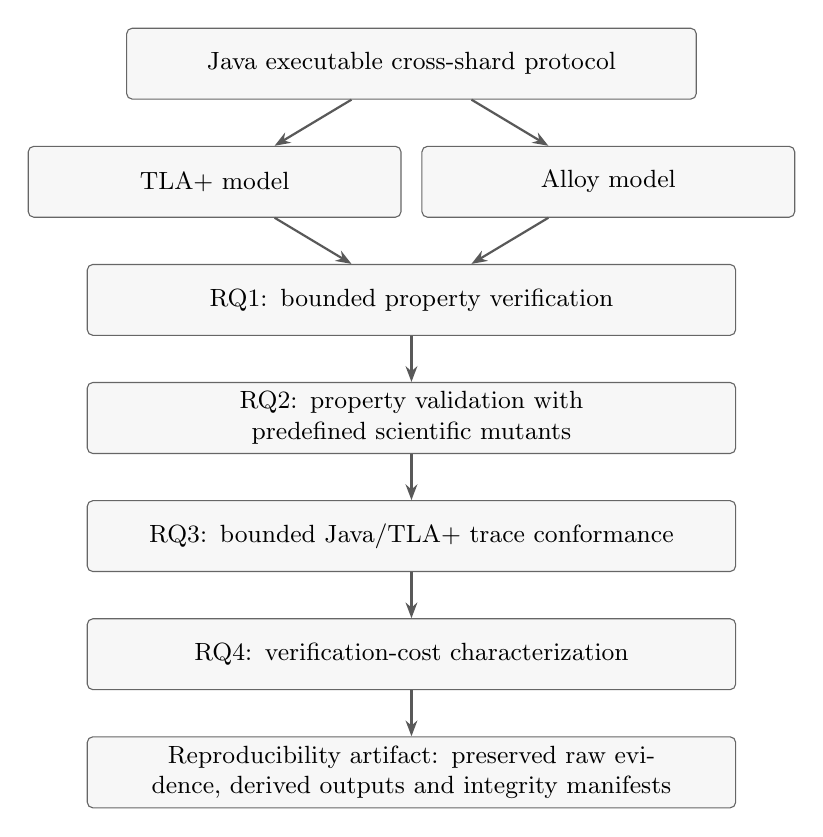
\begin{tikzpicture}[
  box/.style={draw=black!60, rounded corners=2pt, fill=black!3,
    align=center, text width=4.5cm, minimum height=0.9cm, font=\small},
  arrow/.style={-{Stealth[length=2mm]}, thick, draw=black!65}]
\node[box,text width=7cm] (java) at (0,0) {Java executable cross-shard protocol};
\node[box] (tla) at (-2.5,-1.5) {TLA+ model};
\node[box] (alloy) at (2.5,-1.5) {Alloy model};
\node[box,text width=8cm] (rq1) at (0,-3) {RQ1: bounded property verification};
\node[box,text width=8cm] (rq2) at (0,-4.5) {RQ2: property validation with predefined scientific mutants};
\node[box,text width=8cm] (rq3) at (0,-6) {RQ3: bounded Java/TLA+ trace conformance};
\node[box,text width=8cm] (rq4) at (0,-7.5) {RQ4: verification-cost characterization};
\node[box,text width=8cm] (artifact) at (0,-9) {Reproducibility artifact: preserved raw evidence, derived outputs and integrity manifests};
\draw[arrow] (java) -- (tla);
\draw[arrow] (java) -- (alloy);
\draw[arrow] (tla) -- (rq1);
\draw[arrow] (alloy) -- (rq1);
\draw[arrow] (rq1) -- (rq2);
\draw[arrow] (rq2) -- (rq3);
\draw[arrow] (rq3) -- (rq4);
\draw[arrow] (rq4) -- (artifact);
\end{tikzpicture}
\caption{Organization of the complementary evidence layers under the frozen
experimental protocol. Arrows organize the evidence workflow, not formal
refinement, model equivalence, or cumulative proof. TLA+ and Alloy are parallel
representations. RQ4 reuses the RQ1 bound-profile measurements and additional
TLC fault-profile measurements.}
\label{fig:evidence-workflow}
\end{figure}


The design was frozen before the definitive experimental campaign. Research
questions, hypotheses, factors, configuration profiles, seeds, repetitions,
resource limits, statistical procedures, and rules for incomplete executions
were specified before observing the final results. Changes to these elements
after inspection of the definitive outcomes would require a new protocol
version.

\subsection{Research questions and hypotheses}
\label{subsec:research-questions}

\paragraph{RQ1: Preservation of declared properties}

Does the cross-shard commit protocol preserve the declared properties under the
explored interleavings within the documented bounds?

The corresponding hypothesis is:

\begin{quote}
\textbf{H1.} Valid models produce no property violations within the declared
bounds.
\end{quote}

RQ1 is interpreted only for the executed property, tool, configuration, and
bound, not as an unbounded correctness proof.

\paragraph{RQ2: Defect-detection capability}

Do TLC and Alloy detect predefined scientific mutations that remove controls
from the cross-shard protocol?

The corresponding hypothesis is:

\begin{quote}
\textbf{H2.} Each scientific mutant produces a violation of its designated
target property.
\end{quote}

Detection requires the designated target property to be reported among the
violations, although a mutant may violate additional properties.

\paragraph{RQ3: Bounded implementation-model trace conformance}

Do projected traces from the Java simulator and deliberately mutated abstract
traces produce the expected bounded TLC replay outcomes?

The corresponding hypothesis is:

\begin{quote}
\textbf{H3.} Valid traces are accepted and corrupted traces are rejected at the
expected point.
\end{quote}

RQ3 provides bounded implementation-model trace-conformance evidence rather
than a general refinement proof or behavioral equivalence.

\paragraph{RQ4: Verification cost}

How does verification cost change as the number of shards, concurrent
transfers, bounds, and enabled faults increase?

The preregistered hypothesis is:

\begin{quote}
\textbf{H4.} Model-checking cost grows nonlinearly with the number of concurrent
transfers and shards.
\end{quote}

H4 is empirical rather than assumed and is evaluated from observed
profile-level cost measurements.

\subsection{Methodological layers}
\label{subsec:methodological-layers}

The four questions form three verification and validation layers plus one
cost-analysis layer.

\subsubsection{Bounded property-verification layer}

RQ1 evaluates the valid TLA+ and Alloy specifications against the seven
protocol properties in Section~\ref{subsec:properties}. The experimental unit
consists of:

\begin{itemize}
\item a protocol property
\item a formal tool
\item a bounded configuration
\item a measured repetition
\end{itemize}

Response variables include property outcome, available state-space information,
exploration depth or scope, elapsed time, maximum resident memory, exit status,
and counterexample information. A completed execution without a counterexample
provides evidence only within its declared finite configuration. Timeout and
out-of-memory outcomes remain incomplete or censored observations.

\subsubsection{Mutation-based property validation layer}

RQ2 evaluates scientific mutants that remove specific protocol controls:
replay protection, receipt-dependent destination credit, terminal-decision
consistency, timeout release of source funds, and quorum enforcement. The
experimental unit consists of:

\begin{itemize}
\item a scientific mutant
\item a formal tool
\item a bounded configuration
\item a measured repetition
\end{itemize}

Each mutant has one predefined target property, and detection is credited only
when that property is violated. The aggregate measure is

\begin{equation}
\mathrm{MutationScore}
=
\frac{N_{\mathrm{detected}}}
{N_{\mathrm{mutants}}},
\label{eq:mutation-score}
\end{equation}

where \(N_{\mathrm{detected}}\) is the number of predefined mutants detected
through their target properties and \(N_{\mathrm{mutants}}\) is the number
evaluated. The score applies only to the predefined catalogue and does not
establish property-suite completeness.

\subsubsection{Bounded implementation-model trace-conformance layer}

RQ3 evaluates deterministic Java traces projected through the Java-to-TLA+
abstraction in Section~\ref{subsec:formal-abstraction}. The experimental unit
consists of:

\begin{itemize}
\item a valid scenario or negative mutation
\item a deterministic seed
\item the corresponding TLC replay outcome
\end{itemize}

Two trace classes are evaluated: positive projections of simulated Java
scenarios and negative controls obtained by mutating already projected
abstract traces. The latter do not represent Java code defects. A valid trace is classified successfully when its projected action
sequence is admitted by the replay model. A corrupted trace succeeds
experimentally when it is rejected at the predefined diagnostic point.

For negative traces, the observed diagnostic must also agree with the expected
abstract step, concrete step, action, and transfer identifier. These criteria
distinguish generic replay failure from rejection at the intended protocol
location. The evidence remains bounded to the frozen scenario, mutation, seed,
and projection catalogue.

\subsubsection{Verification-cost characterization layer}

RQ4 characterizes bounded verification cost. The experimental unit consists of:

\begin{itemize}
\item a formal tool
\item a bound profile
\item a fault profile when applicable
\item a measured repetition
\end{itemize}

Response variables are elapsed time, maximum resident memory, generated and
distinct states when available, exploration depth or Alloy scope, timeout,
out-of-memory outcome, and within-tool growth ratios. Because TLC and Alloy
expose different exploration semantics and state representations, cost trends
are analyzed within each tool rather than by treating their absolute
measurements as interchangeable.

\subsection{Triangulation of evidence}
\label{subsec:evidence-triangulation}

The layers address different weaknesses in the scientific argument. RQ1
evaluates bounded property outcomes but cannot show by itself that the
properties expose relevant defects. RQ2 adds targeted defect sensitivity.
Formal-model evidence alone does not establish agreement with the executable
implementation, so RQ3 adds bounded trace conformance with positive and
negative cases. RQ4 characterizes the computational envelope in which the
formal evidence is obtained.

The dependency among the layers is deliberate. Successful bounded checking in
RQ1 is more informative when RQ2 shows that selected weakened controls trigger
their target properties. Those two layers remain statements about formal
representations, so RQ3 confronts the abstraction with executable traces. RQ4
then reports the resource envelope within which the formal evidence was
obtained.

Thus, the first three layers provide complementary evidence about bounded
property outcomes, defect sensitivity, and implementation-model trace
conformance, while the fourth characterizes their verification cost. The layers
strengthen different parts of the argument, but no layer is interpreted as
replacing the limitations of another.

\subsection{Treatment of incomplete executions}
\label{subsec:incomplete-executions}

Experimental outcomes are retained according to observed status.
Counterexamples, timeouts, out-of-memory results, and other scientifically
meaningful unfavorable outcomes are not removed. A failed instrumentation
attempt may be repeated only under the predefined protocol rules, not because a
run produced an unexpected scientific result.

Timeout and out-of-memory observations are retained as censored results rather
than assigned artificial elapsed-time or memory values or reclassified as
successful verification. This prevents incomplete runs from being converted
into positive evidence.

\subsection{Interpretation boundaries}
\label{subsec:method-boundaries}

All claims remain bounded by the declared protocol model, properties,
configurations, scopes, scenarios, seeds, mutant catalogue, and execution
environment. Absence of a counterexample is not an unrestricted proof,
mutation analysis does not establish property-suite completeness, and trace
replay does not establish general refinement or behavioral equivalence. TLC and
Alloy have different semantics and cost units, so their absolute measurements
do not establish intrinsic tool superiority. The evaluated configurations are
abstractions rather than unrestricted production blockchain systems.

% Auditoría post hoc, distinta del protocolo 8A congelado.
\subsection{Post-campaign evidence audit and claim attribution}
\label{subsec:evidence-audit-method}

An additional analysis was undertaken \emph{after} the V1 protocol had been
frozen and executed. It does not replace the four preregistered research
questions or alter their denominators. The audit reviews the original model
predicates and Java transitions, decomposes the fourteen frozen experiment
families, and classifies the independently preserved G3 Java mutation logs.
Each assertion is associated with one of four evidence types: (i) TLC/Alloy
checks of a finite formal model, (ii) executions of the Java simulator,
(iii) mutation of already projected abstract traces, or (iv) regeneration
of outputs from immutable raw measurements. An observation is not promoted
to a proof at a higher abstraction level without a documented semantic
connection and corresponding witness or checker outcome.

The audit explicitly allows inconclusive outcomes: timeout, compilation
failure, mutation survival, inaccessible raw results, and unspecified
refinement are not silently recoded as success. For Java mutations, evidence
records activation, compilation, the focal test result, test dependencies,
and the earliest observable failure; the test exit code alone does not
identify causal detector sensitivity. Repetition in an unchanged
model/bound or scenario/seed family is kept distinct from independent defect
classes. This audit is an interpretation of preserved empirical records and
source code; it does not constitute a new preregistered effectiveness trial.


\section{Experimental Design}
\label{sec:experimental-design}

\subsection{Frozen experimental protocol}
\label{subsec:frozen-protocol}

The definitive experiment follows protocol \texttt{paper1-q3-v1}, frozen before
execution of the experimental matrix. It specifies the research questions,
hypotheses, configuration families, seeds, repetitions, resource limits,
statistical procedures, and treatment of incomplete executions.

The scientific baseline corresponds to release \texttt{v1.1.0-rc.1}. The frozen
toolchain consists of TLA+ Tools 1.7.4, Alloy 6.2.0 with SAT4J, Java 17,
Python 3.12, and GNU \texttt{/usr/bin/time -v} for time and memory
instrumentation.

The definitive design covers bounded property verification, scientific mutants,
bounded implementation-model trace conformance, and TLC fault profiles.
Configuration families were enumerated before definitive execution. No
configuration absent from the frozen matrix was added after observing outcomes.

\subsection{Configuration matrix}
\label{subsec:configuration-matrix}

The experimental matrix contains fourteen configuration families:

\begin{itemize}
\item six valid-model scalability families, with small, medium, and large
profiles for TLC and Alloy
\item two mutation families, one per formal tool
\item two trace-conformance families, valid and negative
\item four TLC fault-profile families covering normal execution, replay
pressure, timeout behavior, and a unanimity threshold
\end{itemize}

Table~\ref{tab:all-configuration-families} identifies each frozen family and its
contribution to the task count, including separately recorded warm-up and
measured executions. Each identifier corresponds to the configuration ledger
in \texttt{experiments/paper1/configurations.csv}; the full scenario and
property catalogs are given in \texttt{experiments/paper1/cases.json}.
% Desglose reproducible de las catorce familias del protocolo V1.
% Fuente: experiments/paper1/configurations.csv y cases.json.
% Solo presenta el plan; NO valida los resultados raw.
\begin{table}[htbp]
\centering
\scriptsize
\setlength{\tabcolsep}{2pt}
\caption{All fourteen frozen configuration families. Counts distinguish scheduled warm-ups from measured executions. The identifiers match \texttt{configurations.csv}.}
\label{tab:all-configuration-families}
\begin{tabular}{p{0.39\linewidth}p{0.19\linewidth}rrr}
\hline
Configuration ID & Expansion & Tasks & Warm-up & Measured \\
\hline
\texttt{RQ1R4-TLC-SMALL} & 7 properties & 84 & 14 & 70 \\
\texttt{RQ1R4-TLC-MEDIUM} & 7 properties & 84 & 14 & 70 \\
\texttt{RQ1R4-TLC-LARGE} & 7 properties & 84 & 14 & 70 \\
\texttt{RQ1R4-ALLOY-SMALL} & 7 properties & 84 & 14 & 70 \\
\texttt{RQ1R4-ALLOY-MEDIUM} & 7 properties & 84 & 14 & 70 \\
\texttt{RQ1R4-ALLOY-LARGE} & 7 properties & 84 & 14 & 70 \\
\texttt{RQ2-TLC-MUTANTS} & 5 mutants & 60 & 10 & 50 \\
\texttt{RQ2-ALLOY-MUTANTS} & 5 mutants & 60 & 10 & 50 \\
\texttt{RQ3-TLC-VALID} & 10 cases, 30 seeds & 300 & 0 & 300 \\
\texttt{RQ3-TLC-NEGATIVE} & 10 cases, 30 seeds & 300 & 0 & 300 \\
\texttt{RQ4-TLC-FAULT-NORMAL} & 1 fault profile & 12 & 2 & 10 \\
\texttt{RQ4-TLC-FAULT-REPLAY} & 1 fault profile & 12 & 2 & 10 \\
\texttt{RQ4-TLC-FAULT-TIMEOUT} & 1 fault profile & 12 & 2 & 10 \\
\texttt{RQ4-TLC-FAULT-QUORUM} & 1 fault profile & 12 & 2 & 10 \\
\hline
\textbf{Total} & 14 families & \textbf{1272} & \textbf{112} & \textbf{1160} \\
\hline
\end{tabular}
\end{table}


In particular, the six valid-model families account for 504 tasks, the two
formal mutation families for 120, the two conformance families for 600,
and the four TLC fault-profile families for 48, totaling 1272. Exactly 112
are warm-ups and 1160 are measured observations. These are the frozen V1
schedule counts, not results of the subsequent V2.2 pilot.

These families expand through properties, mutants, repetitions, scenarios, and
seeds into 1272 scheduled tasks. The count includes warm-up and measured
executions where defined, while RQ3 contributes one replay execution per
case-seed pair.

Each task records protocol and configuration identifiers, tool, model kind,
profile, repetition or seed, resource limits, and provenance metadata.

\subsection{Bound profiles}
\label{subsec:bound-profiles}

Three ordered profiles define the principal bounded scalability configurations
in Table~\ref{tab:bound-profiles}.

\begin{table}[htbp]
\centering
\footnotesize
\setlength{\tabcolsep}{2pt}
\caption{Bound profiles used in the definitive experiment.}
\label{tab:bound-profiles}
\begin{tabular}{lrrrrrrr}
\hline
\noalign{\vskip 3pt}
Profile &
Shards &
Transfers &
Validators &
\shortstack{TLC\\quorum} &
\shortstack{TLC receipt\\copies} &
\shortstack{Alloy Receipt\\scope} &
\shortstack{Alloy State\\scope} \\
\hline
Small  & 2 & 1 & 2 & 2 & 1 & 2 & 6  \\
Medium & 3 & 2 & 3 & 2 & 2 & 4 & 8  \\
Large  & 4 & 3 & 4 & 3 & 2 & 6 & 10 \\
\hline
\end{tabular}
\end{table}

Shard, transfer, and validator counts are shared across the profile records.
TLC quorum and receipt-copy columns are TLC parameters. Alloy instead uses
Receipt scopes 2, 4, and 6, Message scopes 10, 20, and 30, and State scopes
6, 8, and 10 for small, medium, and large. Its commit predicate requires at
least two votes in every profile, so TLC quorum values are not Alloy quorum
thresholds.

Profiles are experimental bundles, not one-factor perturbations: shared
configuration sizes and tool-specific bounds vary together. Cost changes are
therefore associated with the complete profile rather than attributed causally
to one parameter. The \texttt{catalog} profile is reserved for RQ3 scenarios.

\subsection{Mutation configurations}
\label{subsec:mutation-configurations}

Mutation experiments use the medium profile. Five scientific defect classes are
instantiated for each formal representation:

\begin{itemize}
\item removal of receipt replay protection
\item destination credit before valid receipt consumption
\item commit after an abort-like terminal decision
\item timeout without release of source funds
\item quorum bypass
\end{itemize}

Each mutant has a predefined target property. After two warm-ups, ten measured
repetitions are executed per mutant, and logical detection must remain
consistent across measured repetitions.

\subsection{Trace-conformance configurations}
\label{subsec:trace-configurations}

RQ3 uses a separate multiseed design with ten valid scenarios and ten negative
cases. Each case is evaluated under thirty deterministic seeds, producing
300 valid and 300 negative trace executions. The definitive seed sequence is
\texttt{2026001} through \texttt{2026030}.

RQ3 therefore contains 600 TLC replay executions. Each case-seed pair executes
once without warm-up because the primary outcome is deterministic
classification, not repeated performance estimation.

\subsection{Repetitions and execution order}
\label{subsec:repetitions}

Model-checking configurations used for time and memory measurement have two
warm-up repetitions, ten measured repetitions, serial execution, and exclusion
of warm-ups from primary statistical analysis. Warm-up observations remain in
the execution record but do not contribute to the reported cost summaries.

Logical outcomes are expected to remain consistent across repetitions.
Repetition characterizes elapsed time and memory rather than creating
independent logical property outcomes. No run is repeated because it produces a
counterexample, timeout, or other unfavorable scientific result.

\subsection{Resource limits}
\label{subsec:resource-limits}

Each measured model-checking execution uses:

\begin{itemize}
\item timeout: 1800 seconds
\item maximum resident-memory limit: 12288 MiB
\item maximum concurrent experimental executions: one
\item TLC workers: one
\item Alloy solver: SAT4J
\end{itemize}

Time and maximum resident memory are collected with
\texttt{/usr/bin/time -v}. Timeout and out-of-memory outcomes remain
scientifically meaningful scalability observations in the experimental record
and are not removed from the matrix.

\subsection{Execution environment}
\label{subsec:execution-environment}

The definitive timing and memory campaign runs on a dedicated native Linux host.
Virtualized environments, WSL, and shared continuous-integration runners are
excluded from primary timing and memory measurements. Continuous integration is
used for functional, structural-integrity, and reproducibility checks, but its
timings are not mixed with definitive performance measurements.

Recorded environment metadata includes operating system and kernel, processor
architecture and count, available memory, Java and Python versions, formal-tool
versions, repository commit, and virtualization status.

\subsection{Measured outcomes}
\label{subsec:measured-outcomes}

For TLC, recorded measurements include:

\begin{itemize}
\item property result
\item generated states
\item distinct states
\item exploration depth
\item elapsed time
\item maximum resident memory
\item process exit status
\item counterexample information when applicable
\end{itemize}

For Alloy, recorded measurements include:

\begin{itemize}
\item assertion result
\item solver and scope
\item counterexample information
\item solving and total elapsed time when available
\item maximum resident memory
\item process exit status
\end{itemize}

TLC state counts and Alloy scopes are not equivalent state-space units.

Trace-conformance records include case identifier, seed, case type, acceptance
or rejection, diagnostic agreement, abstract and concrete steps, action,
transfer identifier, elapsed time, memory, source commit, and input hashes.

\subsection{Incomplete executions and censoring}
\label{subsec:censoring}

Executions may terminate as completed runs, counterexamples, timeouts,
out-of-memory outcomes, tool errors, or instrumentation failures. Timeout and
out-of-memory outcomes are retained as censored observations without replacing
their elapsed-time or memory values by configured limits or synthetic values.

Unexpected tool exits remain tool errors. Instrumentation failures may be
retried only under the frozen retry policy and never on the basis of the
scientific result. This treatment preserves unfavorable outcomes and prevents
selective removal of executions that would weaken a hypothesis.

\subsection{Statistical analysis}
\label{subsec:statistical-analysis}

Time and memory distributions are summarized by median and interquartile range,
with minimum, maximum, and coefficient of variation also retained. A 95\%
bootstrap confidence interval for the median uses 10,000 resamples. Wilson 95\%
confidence intervals are used for proportions, including mutation detection and
trace classification.

RQ4 reports profile-level medians and within-tool growth ratios. Spearman rank
association describes monotonic association between ordered profile and cost
when sufficient completed profiles are available.

TLC and Alloy are not compared through absolute execution-time claims because
their modelling semantics and state-space representations differ. Such
measurements are not treated as evidence of intrinsic tool superiority. The
three ordered profiles provide descriptive bounded-cost evidence but do not
establish an asymptotic complexity class or a general nonlinear growth law.

% Basado en experiments/paper1/configurations.csv y cases.json congelados.
\subsection{Exhaustive definition of the fourteen experimental families}
\label{subsec:individual-families}

The frozen study uses fourteen configuration-family identifiers, not fourteen
independent protocol implementations. Table~\ref{tab:family-detail} reports
the exact scheduled unit counts; the raw observations are linked to individual
\texttt{task\_id} records rather than inferred from this table. A model
configuration repeated for performance estimation remains one logical
property/bound question, not ten independent proofs.

\begin{table}[htbp]
\centering
\scriptsize
\setlength{\tabcolsep}{3pt}
\caption{Exhaustive frozen experiment plan; counts include only tasks defined
by \texttt{paper1-q3-v1}.}
\label{tab:family-detail}
\begin{tabular}{@{}llrr@{}}
\hline
Family ID & Unit repeated & Warm-up & Measured \\
\hline
\texttt{RQ1R4-TLC-SMALL} & 7 property checks & 14 & 70 \\
\texttt{RQ1R4-TLC-MEDIUM} & 7 property checks & 14 & 70 \\
\texttt{RQ1R4-TLC-LARGE} & 7 property checks & 14 & 70 \\
\texttt{RQ1R4-ALLOY-SMALL} & 7 assertion checks & 14 & 70 \\
\texttt{RQ1R4-ALLOY-MEDIUM} & 7 assertion checks & 14 & 70 \\
\texttt{RQ1R4-ALLOY-LARGE} & 7 assertion checks & 14 & 70 \\
\texttt{RQ2-TLC-MUTANTS} & 5 formal mutants & 10 & 50 \\
\texttt{RQ2-ALLOY-MUTANTS} & 5 formal mutants & 10 & 50 \\
\texttt{RQ3-TLC-VALID} & 10 cases $\times$ 30 seeds & 0 & 300 \\
\texttt{RQ3-TLC-NEGATIVE} & 10 abstract mutations $\times$ 30 seeds & 0 & 300 \\
\texttt{RQ4-TLC-FAULT-NORMAL} & 1 fault profile & 2 & 10 \\
\texttt{RQ4-TLC-FAULT-REPLAY} & 1 fault profile & 2 & 10 \\
\texttt{RQ4-TLC-FAULT-TIMEOUT} & 1 fault profile & 2 & 10 \\
\texttt{RQ4-TLC-FAULT-QUORUM} & 1 fault profile & 2 & 10 \\
\hline
Total & 14 families & 112 & 1160 \\
\hline
\end{tabular}
\end{table}

\paragraph{Six bounded property families.}
Each of the seven V1 properties is checked separately on TLC and Alloy for
small, medium and large profiles, with two warm-ups and ten measured runs per
property. The profiles increase from two shards, one transfer and two
validators, through three shards, two transfers and three validators, to
four shards, three transfers and four validators. TLC quorum is respectively
2, 2 and 3 and receipt copies are 1, 2 and 2. All three base TLC profiles set
\texttt{EnableTimeout=FALSE}. In the correct V1 model this disables the only
route to \texttt{Aborted}, so the implication
\(\texttt{Aborted}\Rightarrow\texttt{fundsReleased}\) holds vacuously in
completed base TLC checks. The censored large profile yields no completed
verdict. Alloy uses exactly 6, 8 and 10
state atoms, with respectively 2, 4 and 6 receipt atoms and 10, 20 and 30
message atoms. Unlike TLC-large, the frozen Alloy commit condition remains
at least two votes. Thus cross-tool profile labels are not isomorphic and
absolute runtime or state-space comparisons would be invalid.

\paragraph{Two formal mutation families.}
The five TLC and five Alloy model mutations remove controls for receipt
replay, credit without receipt, commit after abort, timeout without release,
and quorum bypass. Their predefined target properties are evaluated ten times
per formal mutant, following two warm-ups. These are ten \emph{formal model}
mutants, not Java code mutants; repeated checker executions are not new
defect definitions. Mutation selection directly targets guards, which limits
its value as evidence of broadly adequate safety specifications.

\paragraph{Two replay families.}
The valid population consists of ten deterministic Java-simulator scenarios
projected to V1 TLA+, each run with thirty distinct seeds (2026001--2026030).
The negative population consists of ten deliberately altered \emph{abstract}
traces derived from simulator scenarios and replayed under the same seeds.
The negative cases therefore test rejection of abstract-step violations, not
the detection of 300 independently introduced Java implementation faults.
Neither population has warm-up repetitions. The mapping canonicalizes
approval counts into synthetic validator identities and maps certain network
observations to stuttering actions.

\paragraph{Four TLC cost/fault families.}
The frozen medium-base model is separately evaluated with: (i) normal
execution, one receipt copy and timeout disabled; (ii) replay pressure, two
copies and timeout disabled; (iii) two copies, timeout enabled and copy 1 delayed; and
(iv) Unanimity (3 of 3), with two receipt copies, no delayed copies and
timeout disabled. All three validators remain eligible to vote. The historical
identifiers are \texttt{RQ4-TLC-FAULT-QUORUM} and
\texttt{fault-insufficient\_quorum}. Each family
checks one fixed property, with two warm-ups and ten measurements. The
normal and replay profiles target \texttt{NoReceiptReplay}, the timeout
profile targets the historical state invariant
\texttt{EventuallyReleasedAfterTimeout}, and the quorum profile targets
\texttt{QuorumRequired}. Fault-profile cost differences are conditional on
these settings, not causal effects of a single independently varied factor.

\paragraph{Censoring and provenance.}
Every measured formal-tool invocation is bounded by 1800 seconds, 12288 MiB
RSS, and serial execution. The historical analysis reports 70 measured
TLC-large timeouts among the RQ1 checks; they remain censored, not completed
verifications. The complete run is defined by 112 warm-ups and 1160 measured
tasks, and requires a one-to-one mapping from the plan to all 1272
\texttt{result.json} files and their logs. Availability of a matching derived
CSV or analysis hash alone is insufficient to certify that mapping.


\section{Results}
\label{sec:results}

\subsection{Experimental campaign overview}
\label{subsec:results-overview}

The definitive campaign contained 1272 scheduled experimental tasks
across the four research questions. This section reports only measured
runs when evaluating the research hypotheses; warm-up executions are
reported separately from the principal statistical evidence.

Results follow RQ1--RQ4, with incomplete executions retained under the
censoring policy in Section~\ref{subsec:censoring}. To trace an aggregate
to the archived records, use the configuration family, property or case,
and repetition or seed in \path{reference/derived/task-results.csv}.
RQ1 and the bound-profile part of RQ4 share the six tool--bound families.
RQ2 selects the two model-mutant families by target property, RQ3 selects
the two replay families by case and seed, and the additional TLC cost
table uses the four \texttt{RQ4-TLC-FAULT-*} families. Each row links to
the original task record. Section~\ref{subsec:artifact-access} gives the
file paths.

\subsection{RQ1: Bounded property verification}
\label{subsec:rq1-results}

RQ1 reports the seven declared properties for valid formal models within
the evaluated bounds.

Across both formal tools and the three bound profiles, RQ1 contained
420 measured property runs. Of these, 350 completed and 70 were
censored by timeout. No completed run produced a counterexample.

Table~\ref{tab:rq1-summary} summarizes results by tool and profile.

\begin{table}[htbp]
\centering
\caption{RQ1 bounded property-verification results by tool and profile.}
\label{tab:rq1-summary}
\begin{tabular}{llrrrr}
\hline
Tool & Profile & Measured & Completed & No counterexample & Timeout \\
\hline
Alloy & Small  & 70 & 70 & 70 & 0  \\
Alloy & Medium & 70 & 70 & 70 & 0  \\
Alloy & Large  & 70 & 70 & 70 & 0  \\
TLC   & Small  & 70 & 70 & 70 & 0  \\
TLC   & Medium & 70 & 70 & 70 & 0  \\
TLC   & Large  & 70 & 0  & 0  & 70 \\
\hline
Total &        & 420 & 350 & 350 & 70 \\
\hline
\end{tabular}
\end{table}

For Alloy, all seven properties completed without a counterexample
under the small, medium, and large profiles. Each property-profile
combination was measured ten times, yielding 210 completed Alloy runs.

For TLC, all seven properties completed without a counterexample under
the small and medium profiles, yielding 140 completed runs. In
contrast, every measured execution under the large TLC profile reached
the predefined 1800-second timeout. This produced 70 censored
observations, corresponding to seven properties and ten measured
repetitions per property.

The base TLC configurations set \texttt{EnableTimeout=FALSE}. The correct
model therefore cannot reach \texttt{Aborted} in these profiles. The ten
completed \texttt{EventuallyReleasedAfterTimeout} checks in each of TLC-small
and TLC-medium satisfy \(\texttt{Aborted}\Rightarrow\texttt{fundsReleased}\)
vacuously. These 20 checks remain in the historical totals. The timeout-enabled
TLC family exercises the abort branch and its release invariant. The
\texttt{TimeoutWithoutRelease} mutant tests sensitivity to omission of release.
The seven TLC-large property combinations remain censored.

No out-of-memory or tool-error outcome was observed in the RQ1
measurements. The incomplete evidence is therefore concentrated
entirely in the large TLC profile.

\paragraph{Unit of analysis, repetitions, and independent claims.}
The 420 RQ1 measured executions are ten serial repetitions of each of 42
unique tool--property--bound combinations (two tools, seven properties,
three profiles). Thus, 350 completed invocations correspond to 35 completed
combinations; the 70 TLC-large timeouts correspond to seven entirely censored
combinations. Repetitions describe timing and resource variability; they are
not 350 independent specifications or demonstrations of general correctness.
The ten RQ2 mutant definitions, each repeated ten times, are also not 100
independent defect classes. RQ3 includes 20 predefined trace classes tested
with 30 deterministic seeds each, and the negative classes are modifications
of already projected abstract traces, not separately injected Java bugs.
All outcome counts below are preserved as reported; the retrospective audit
changes their interpretation, not their underlying recorded values.

\subsubsection{Answer to RQ1}
\label{subsubsec:rq1-answer}

Within the 350 completed bounded model-checking runs, no violation of
the seven evaluated properties was observed. This provides supporting
evidence for H1 within the completed configurations, subject to the
vacuous base TLC timeout-release checks described above.

However, the 70 large-profile TLC measurements did not complete within
the predefined resource limit. Their absence of a counterexample
cannot be interpreted as successful property verification.

H1 is therefore partially supported under censoring. The result is
restricted to the completed bounded configurations and does not
constitute an unbounded proof of protocol correctness.

\subsection{RQ2: Mutation-based property validation}
\label{subsec:rq2-results}

RQ2 tests whether predefined scientific mutants expose their designated
property violations.

The experiment contained ten scientific mutants: five instantiated in
the TLA+ model and five in the Alloy model. Each mutant was evaluated
through ten measured repetitions at the medium profile, producing 100
measured mutation runs.

All ten scientific mutants were detected through their designated
target properties, and detection remained consistent across all
measured repetitions. The resulting mutation score was

\begin{equation}
\mathrm{MutationScore}
=
\frac{10}{10}
=
1.0.
\label{eq:rq2-mutation-score}
\end{equation}

Table~\ref{tab:rq2-summary} summarizes the aggregate result.

\begin{table}[htbp]
\centering
\footnotesize
\setlength{\tabcolsep}{2pt}
\caption{RQ2 scientific mutants, target properties, and detection results.}
\label{tab:rq2-summary}
\begin{tabular}{lp{0.23\textwidth}p{0.39\textwidth}cr}
\hline
Tool & Mutant & Target property & Detected & Runs \\
\hline
Alloy &
commit-after-abort &
TerminalState\allowbreak Irreversibility &
Yes & 10/10 \\

Alloy &
credit-before-receipt &
DestinationCreditRequires\allowbreak ValidReceipt &
Yes & 10/10 \\

Alloy &
no-replay &
NoReceipt\allowbreak Replay &
Yes & 10/10 \\

Alloy &
quorum-bypass &
Quorum\allowbreak Required &
Yes & 10/10 \\

Alloy &
timeout-without-release &
EventuallyReleasedAfter\allowbreak Timeout &
Yes & 10/10 \\

TLC &
commit-after-abort &
Decision\allowbreak Consistency &
Yes & 10/10 \\

TLC &
credit-before-receipt &
DestinationCreditRequires\allowbreak ValidReceipt &
Yes & 10/10 \\

TLC &
no-replay &
NoReceipt\allowbreak Replay &
Yes & 10/10 \\

TLC &
quorum-bypass &
Quorum\allowbreak Required &
Yes & 10/10 \\

TLC &
timeout-without-release &
EventuallyReleasedAfter\allowbreak Timeout &
Yes & 10/10 \\
\hline
\end{tabular}
\end{table}

The commit-after-abort defect is associated with different designated
target properties in the two formal representations:
\texttt{TerminalState\allowbreak Irreversibility} in Alloy and
\texttt{Decision\allowbreak Consistency} in TLA+. This difference follows the
tool-specific encodings of terminal consistency and does not affect
the mutant-level detection criterion.

The evaluated defect classes covered removal of replay protection,
destination credit without the required receipt condition, commit after
an abort-like terminal decision, timeout without release of source
funds, and quorum bypass.

Detection was evaluated at the mutant level rather than by counting
individual counterexample-producing repetitions as separate mutants.
Therefore, the 100 measured runs represent repeated evaluations of ten
scientific mutants, not 100 independent mutant definitions.

The repeated measurements also verified consistency of the logical
outcome: each mutant continued to expose its designated target-property
violation across all ten measured repetitions.

No absolute execution-time comparison between TLC and Alloy is used to
support RQ2. The two formal representations have different exploration
semantics, and the relevant result for this research question is
whether each predefined mutant exposes its designated property
violation.

\subsubsection{Answer to RQ2}
\label{subsubsec:rq2-answer}

All ten predefined scientific mutants were detected through their
target properties, yielding a mutation score of 1.0 with consistent
detection across the measured repetitions.

H2 is therefore supported for the predefined scientific mutant
catalogue.

This result demonstrates that the evaluated property suite is
sensitive to the injected defect classes considered in the experiment.
It does not establish completeness with respect to arbitrary
cross-shard protocol defects or mutations outside the predefined
catalogue.

\subsection{RQ3: Bounded implementation-model trace conformance}
\label{subsec:rq3-results}

RQ3 evaluates whether projected Java traces are admitted by the TLA+
model within the predefined scenarios and bounds.

The experiment contained ten valid scenarios and ten deliberately
corrupted negative cases. Each case was executed under thirty
deterministic seeds, producing 600 measured replay executions.

All 300 valid traces were accepted by the bounded replay procedure.
All 300 negative traces were rejected. For every negative execution,
the diagnostic information also identified the expected rejection
point, yielding 300 matching diagnostics.

Table~\ref{tab:rq3-summary} summarizes the aggregate classification
results.

\begin{table}[htbp]
\centering
\caption{RQ3 bounded trace-conformance results.}
\label{tab:rq3-summary}
\begin{tabular}{lrrrr}
\hline
Trace class &
Cases &
Runs &
Correct classification &
Matching diagnostics \\
\hline
Valid    & 10 & 300 & 300 & --  \\
Negative & 10 & 300 & 300 & 300 \\
\hline
Total    & 20 & 600 & 600 & 300 \\
\hline
\end{tabular}
\end{table}

At the individual-case level, every one of the twenty scenarios
obtained 30 correct classifications out of 30 seeds. The observed
classification proportion was therefore 1.0 for every case. The
case-level Wilson 95\% interval associated with 30 successes in 30
runs had a lower bound of approximately 0.8865 and an upper bound of
1.0.

The valid catalogue includes normal commit, timeout-related behavior,
duplicated receipts, delayed delivery after timeout, same-round commit
and timeout, conflicting use of the same UTXO, bidirectional
transfers, temporary target unavailability, insufficient quorum, and
multiple concurrent sessions.

The negative catalogue contains deliberately corrupted traces,
including commit from a pending state, commit after abort, receipt
replay, destination credit without a valid receipt, timeout without
release, commit without quorum, duplicate voting, transfer-identifier
changes, shard-topology changes, and receipt consumption before the
source lock.

The diagnostic criterion is evaluated only for negative cases because
these executions are expected to be rejected at a predefined point.
A matching diagnostic means that the replay procedure rejected the
trace consistently with the expected abstract-action mismatch rather
than merely producing a generic failure.

\paragraph{Distinguishing the sources of positive and negative cases.}
The 300 valid cases originate from ten deterministic Java-simulator
executions under thirty seeds, projected through the V1 abstraction. The
300 negative cases are separately generated by \texttt{NegativeTraceCatalog}
from already projected traces and deliberately altered abstract steps.
They are not 300 faults injected into the Java implementation. Rejection of
those negatives establishes sensitivity to the selected invalid abstract
steps and their expected diagnostic locations, not Java fault-detection
recall. Synthetic canonical validator IDs and receipt copies used by the
projection must not be confused with observed cryptographic identities.

The Wilson interval above is a calculation under a Bernoulli-sampling
interpretation, not a justified coverage bound for the space of future
implementation faults. The 30 seeds are a frozen deterministic set and the
negative classes are hand-defined trace alterations. We therefore use the
proportion only descriptively and do not treat the interval as an inferential
claim about Java bug-detection effectiveness or arbitrary future traces.

\subsubsection{Answer to RQ3}
\label{subsubsec:rq3-answer}

All 300 valid traces were accepted, all 300 deliberately corrupted
traces were rejected, and all 300 negative executions produced the
expected diagnostic agreement.

H3 is therefore supported for the predefined bounded trace catalogue.

This result provides evidence of bounded implementation-model trace
conformance between the Java implementation and the TLA+ abstraction
for the evaluated scenarios and seeds. It does not constitute a
general refinement proof, behavioral equivalence result, or guarantee
that arbitrary Java executions conform to the formal model.

\subsection{RQ4: Bounded verification cost}
\label{subsec:rq4-results}

RQ4 characterizes bounded verification cost across the predefined size
and enabled-fault profiles.

The RQ4 evidence comprises 460 measured executions. Of these, 420
belong to the valid-model small, medium, and large bound profiles
shared with RQ1, and 40 correspond to four additional TLC fault
profiles.

\subsubsection{Cost across bound profiles}
\label{subsubsec:rq4-bound-cost}

Table~\ref{tab:rq4-bound-cost} summarizes time, memory, and profile
outcomes for the three ordered profiles.

\begin{table}[htbp]
\centering
\footnotesize
\setlength{\tabcolsep}{3pt}
\caption{RQ4 cost by formal tool and bound profile.}
\label{tab:rq4-bound-cost}
\begin{tabular}{llrrrrr}
\hline
\noalign{\vskip 3pt}
Tool &
Profile &
Runs &
Completed &
Timeout &
\shortstack{Median time\\(s)} &
\shortstack{Median RSS\\(KiB)} \\
\hline
Alloy & Small  & 70 & 70 & 0  & 0.515306 & 179830 \\
Alloy & Medium & 70 & 70 & 0  & 0.766172 & 299268 \\
Alloy & Large  & 70 & 70 & 0  & 1.568320 & 317612 \\
TLC   & Small  & 70 & 70 & 0  & 0.666802 & 143660 \\
TLC   & Medium & 70 & 70 & 0  & 1.118120 & 601428 \\
TLC   & Large  & 70 & 0  & 70 & --       & --     \\
\hline
\end{tabular}
\end{table}

All Alloy profiles completed. Median elapsed time increased from
0.515306 seconds in the small profile to 0.766172 seconds in the
medium profile and 1.568320 seconds in the large profile. Median
maximum resident memory increased from 179830 KiB to 299268 KiB and
317612 KiB, respectively.

Across the three Alloy profiles, Spearman rank association between the
ordered profile level and both median elapsed time and median maximum
resident memory was 1.0. The large-to-small ratio was approximately
3.043 for median elapsed time and 1.766 for median memory.

For TLC, the small and medium profiles completed, with median elapsed
times of 0.666802 and 1.118120 seconds and median maximum resident
memory values of 143660 and 601428 KiB, respectively. Median distinct
states increased from 14 in the small profile to 24336 in the medium
profile.

The large TLC profile did not yield completed measurements. All 70
measured executions reached the predefined 1800-second timeout.
Consequently, elapsed-time, memory, and state-space medians are not
reported for that profile.

The available TLC measurements exhibit increasing cost from small to
medium, but the two completed profile levels are insufficient for a
meaningful characterization of the shape of the growth curve.
Furthermore, the complete censoring of the large profile prevents a
three-level completed-profile analysis.

\subsubsection{Cost across additional TLC profiles}
\label{subsubsec:rq4-fault-cost}

The additional TLC cost experiment evaluates four medium-bound
configurations. All forty measured executions completed without
timeout, out-of-memory, or tool-error outcomes.

\begin{table}[htbp]
\centering
\small
\caption{RQ4 TLC cost across additional medium-bound profiles.}
\label{tab:rq4-fault-cost}
\begin{tabular}{lrrr}
\hline
Fault profile &
Runs &
Median time (s) &
Median RSS (KiB) \\
\hline
Normal               & 10 & 0.867343 & 379846 \\
Unanimity (3 of 3)  & 10 & 1.068210 & 493370 \\
Replay               & 10 & 1.118420 & 604258 \\
Timeout              & 10 & 1.569610 & 822820 \\
\hline
\end{tabular}
\end{table}

The observed costs differ across the TLC medium-bound configurations. Among the evaluated profiles, the
timeout-oriented case produced the largest median elapsed time and
median memory footprint, while the normal profile produced the
smallest values.

These measurements characterize the evaluated fault profiles only.
They are not interpreted as an ordering that generalizes to arbitrary
failure modes.

\subsubsection{Answer to RQ4}
\label{subsubsec:rq4-answer}

The experiments provide evidence that bounded verification cost
increases as the evaluated configurations grow.

For Alloy, all three ordered profiles completed and both median elapsed
time and median memory increased monotonically with profile level.
For TLC, cost increased between the two completed profiles, while all
large-profile measurements were censored by timeout.

These observations support a descriptive claim of increasing
verification cost. They do not establish the preregistered nonlinear
growth claim in H4. Only three ordered profiles were defined, and TLC
provides completed measurements for only two of them.

Accordingly, H4 remains unconfirmed in its nonlinear form: the
experiment provides evidence of growth without sufficient evidence to
establish a nonlinear or asymptotic growth law.

All cost comparisons are interpreted within each formal tool. The
results do not support claims of absolute performance superiority
between TLC and Alloy because their modelling semantics and
state-space representations differ.

% Análisis post-campaña: los resultados de G3 NO forman parte del protocolo 8A/V1.
\subsection{Post-campaign Java mutation forensics: a separate exploratory result}
\label{subsec:java-g3-forensics}

After the frozen V1 experiment, an independently identifiable G3-v1 diagnostic
campaign applied ten manually defined source-code changes to
\texttt{AtomicCommitProtocol.java}, \texttt{Shard.java} or
\texttt{ShardManager.java}. This was an \emph{exploratory post-campaign}
study: the Java mutations were not preregistered as part of RQ2, and their
results are not included in the 1272 V1 tasks. Its source revision was
\texttt{e4422ae4\allowbreak{}83ab0eb4\allowbreak{}c0af48bb\allowbreak{}b58be1c4\allowbreak{}9c8cf816}; the available
archive preserves 274 SHA-256-checked files and the changes applied to each
mutant.

All ten control tests returned PASS. All ten Java mutants compiled, reached
the altered source in the focal test, and produced a focal failure. Across
all 100 mutant--test executions, 51 were FAIL and 49 PASS. This is a count
of test exits, not a 51\% detection rate, a statistically sampled fault
population, or evidence of independent detector effectiveness.

\begin{table}[htbp]
\centering
\footnotesize
\caption{G3-v1 Java mutants and observed test failures. Each row covers
ten tests across the recorded fixtures.}
\label{tab:g3-full}
\begin{tabular}{@{}lp{0.56\linewidth}r@{}}
\hline
Mutant & Java change and focal observation & FAIL/tests \\
\hline
M02 & Destination output assigned to original owner; wrong beneficiary & 1/10 \\
M03 & Change output assigned to wrong public key; ownership mismatch & 1/10 \\
M04 & Change output inflated by one; total 10000 $\rightarrow$ 10001 & 8/10 \\
M05 & Consumes transfer ID instead of receipt ID; wrong receipt identity & 8/10 \\
M06 & Omits restoration of source UTXO on rollback & 7/10 \\
M07 & Marks the receipt again instead of removing its consumption mark during rollback & 7/10 \\
M08 & Reports successful locking when lock insertion fails. The exactly-one-session acceptance check fails. & 2/10 \\
M09 & Selects origin as destination in the commit plan. Tests report a missing destination UTXO and incorrect per-shard deltas. & 9/10 \\
M10 & Omits restoration of the destination output during rollback & 7/10 \\
M11 & Removes synchronization from joint shard read; reader accesses early & 1/10 \\
\hline
\end{tabular}
\end{table}

M02 and M03 each passed the seven historical/G1/G2 tests in the G3-v1
battery. The \texttt{G3\_RECIPIENT} fixture used distinct source owner and
beneficiary keys. On each of the same mutated Java attempts, the
ledger-journal audit printed \texttt{DIVERGENTE} and the subsequent UTXO
assertion identified the wrong beneficiary or change owner, respectively.
The seven earlier tests used different fixtures. G2 also uses the G1
journal, so the paired observations in the focal fixture do not establish
independent detector efficacy or a ranking across fixtures.

M04 changed the ledger total from 10000 to 10001. M05 marked the
transfer identifier in place of the receipt identifier. M06, M07 and M10
changed local restoration operations; failed rollback confirmations and
composite ledger assertions have different diagnostic resolution. M08
returned successful locking despite failed insertion, and its contention
tests rejected the exactly-one-acceptance condition. Recorded results do
not identify two successful commits. M09 routed the commit plan to the
source shard. Its focal test failed at the change-output count before
checking ownership. M11 allowed the joint reader to complete before the
writer was released; the assertion fired before inspecting numerical
snapshot consistency.

G3-v2 is a later campaign with a separate same-scenario comparison by
observation dimension. Its results are outside the 110 G3-v1 runs and the
1,272 V1 tasks. Table~\ref{tab:g3-full} uses the G3-v1 matrix and logs only.
Section~\ref{subsec:artifact-two-populations} identifies the archives.

\section{Discussion}
\label{sec:discussion}

\subsection{Bounded verification evidence}
\label{subsec:discussion-bounded-verification}

RQ1 provides bounded evidence that no declared property was violated in the
completed valid-model configurations. The property suite covers distinct
obligations, including replay protection, destination authorization, decision
consistency, value preservation, quorum enforcement, terminal-state
irreversibility, and release after timeout. The completed base TLC
timeout-release checks are vacuous because those profiles disable timeout.
The timeout-enabled family supplies the relevant abort-branch evidence.

The evidential scope is determined by the explored bounds. Alloy completed all
three predefined profiles, whereas TLC-large was fully censored by the frozen
timeout policy. Those timeouts are not property violations; they delimit the
configurations for which bounded verification completed under the available
resource budget.

Accordingly, H1 supports only the absence of observed violations in completed
bounded configurations. It does not extend to unexplored states, censored
TLC-large executions, or an unbounded correctness claim.

TLC and Alloy provide complementary corroboration rather than interchangeable
proofs. Their different formal semantics and state representations prevent
agreement across completed profiles from implying identical explored spaces or
equivalent proofs.

\subsection{Mutation sensitivity and property adequacy}
\label{subsec:discussion-mutation}

RQ2 complements RQ1 by asking whether the declared properties react when
selected protocol controls are removed. All ten predefined scientific mutants
were detected by their designated target properties, producing a mutation score
of 1.0. This makes the valid-model results more informative because controlled
defects in replay protection, receipt-dependent credit, terminal decisions,
timeout release, and quorum enforcement trigger the expected properties.

Tool-specific encodings can express the same defect intention through different
properties. For example, commit after abort is associated with
\texttt{TerminalState\allowbreak Irreversibility} in Alloy and
\texttt{Decision\allowbreak Consistency} in TLA+. The mutant-level conclusion
therefore concerns targeted defect detection, not identical property
formulations across tools.

The perfect mutation score remains restricted to the predefined catalogue. It
does not establish completeness against arbitrary implementation defects,
modelling errors, or other cross-shard failure modes.

RQ1 and RQ2 thus support complementary claims: the declared properties hold in
the completed valid-model configurations, and the evaluated property suite is
sensitive to the selected protocol controls when they are deliberately
weakened.

\subsection{Implementation-model trace conformance}
\label{subsec:discussion-conformance}

RQ3 adds implementation-facing evidence by replaying observable Java traces
against the TLA+ abstraction. The valid catalogue was accepted and the
deliberately corrupted catalogue rejected as expected, connecting the formal
model with the implementation behaviors exercised by the frozen scenarios.

The negative controls strengthen this result because rejection was checked at
the expected diagnostic point rather than treated as a generic replay failure.
This provides evidence that deliberately introduced mismatches are localized at
the intended abstract-action boundary.

The result remains limited to the selected observable abstraction, scenario
catalogue, negative mutations, and frozen seeds. It therefore supports bounded
implementation-model trace conformance rather than a statement about every
possible Java execution.

In particular, this evidence must not be interpreted as a formal
refinement proof or as behavioral equivalence between the Java
implementation and the TLA+ specification. Establishing refinement
would require a stronger semantic relation covering the full relevant
transition systems, whereas the present experiment validates
correspondence for the predefined observable traces.

RQ3 therefore complements internal model checking and mutation analysis by
confronting the formal abstraction with observable implementation executions.

\subsection{Verification cost and scalability}
\label{subsec:discussion-cost}

RQ4 shows that bounded verification is constrained by computational cost as
well as logical outcome. Measurements increase within both formal tools, but
H4 remains unconfirmed in its preregistered nonlinear form.

For Alloy, all three ordered profiles completed, and median elapsed time and
memory increased monotonically from small to medium and large. The Spearman
association of 1.0 for both metrics is consistent with that ordering, but three
ordinal points cannot identify a functional growth law.

TLC exposes a sharper feasibility boundary. The small and medium profiles
completed with increases in elapsed time, memory, and explored state-space size,
whereas all seventy TLC-large measured runs reached the frozen 1800-second
timeout. Complete censoring precludes a completed-run median for the large
profile and a three-level characterization comparable to Alloy. The timeout is
therefore a valid censored observation, not an experimental failure, and
retaining it makes the evaluated verification boundary explicit.

Within the TLC medium-bound configurations, median time and memory varied
across normal, unanimity (three of three), replay, and
timeout-oriented cases, indicating that verification cost depends on behavioral
structure as well as nominal bound size. These differences do not identify a
universal cost ordering, but they show that enabled behavior is part of the
verification envelope.

The evidence supports only a descriptive conclusion that bounded verification
cost increases for the evaluated configurations. It establishes neither a
nonlinear nor an asymptotic growth law. TLC and Alloy also use different
semantics, exploration mechanisms, and internal representations, so absolute
time, memory, or state-space measurements cannot support intrinsic
tool-superiority claims.

\subsection{Cross-layer evidence triangulation}
\label{subsec:discussion-triangulation}

The four research questions are intended to provide complementary evidence
rather than four independent demonstrations of protocol correctness. Each
addresses a different weakness in the validation argument.

RQ1 evaluates whether the declared properties survive the bounded
interleavings explored for valid formal models. Because absence of a
counterexample does not demonstrate sensitivity to relevant defects, RQ2
deliberately weakens selected protocol controls and checks whether their
designated properties detect the resulting violations.

Formal verification and mutation detection still concern formal
representations. RQ3 adds implementation-facing evidence by checking bounded
conformance of observable Java traces against the TLA+ abstraction, together with
deliberately corrupted abstract-trace controls. This connects the formal layer with the
implementation without implying refinement or behavioral equivalence.

RQ4 makes the computational boundary explicit by characterizing verification
cost as the evaluated bounds become more demanding. The observed increase in
cost and complete TLC-large censoring show that the formal evidence is obtained
within a finite resource envelope.

Together, the layers form an evidence chain from bounded property verification
through mutation-based property validation and bounded implementation-model
trace conformance to verification-cost characterization. The chain is
complementary rather than cumulative proof: model checking remains bounded,
mutation analysis remains catalogue-dependent, trace replay remains limited to
the chosen abstraction and scenarios, and cost characterization remains tied to
the evaluated configurations. No layer removes the limitations of another.

The evidence chain consequently cannot be treated as additive assurance.
Bounded model checks, targeted formal mutants, replay of projected Java
scenarios, rejection of mutated abstract traces, and artifact reconstruction
answer different questions. The contribution of this case study is to
identify the resulting inference boundaries and concrete observational gaps,
not to establish a novel general-purpose verification workflow.

% Discusión negativa y límites de novedad; no reivindicar un nuevo algoritmo.
\subsection{When distinct evidence layers fail to support the same claim}
\label{subsec:observation-adequacy}

The case study yields a falsifiable interpretation of cross-layer evidence:
a successful check supports only the claim expressible by the state
representation, test input, and observation function actually used. This
matters even if all reported verifiers return their expected outcomes.

\paragraph{Ownership cannot be certified by amount-only observation.}
Consider a UTXO ledger state $L$ and a state $L'$ differing only in the
recipient of one existing output, with identical output amounts and shard
assignments. Let $V_s(L)$ be the sum of output amounts in shard $s$. Then
\[
 \forall s:\quad V_s(L)=V_s(L'),
 \qquad\text{although}\qquad L\ne L'.
\]
Any deterministic detector whose only input is the vector
$(V_s(L))_s$ returns the same result for both states. This is a basic
indistinguishability observation, not a new verification theorem. It explains
why ownership-preserving observations are necessary to assert recipient
correctness. The M02/M03 Java executions provide concrete examples of
wrong-recipient outcomes, while the G2 ledger-journal audit reports divergence on the same
beneficiary-distinguishing attempts. The empirical finding
is about what the original workload omitted, not a general weakness of G2.

\paragraph{Boundary correspondence is not internal refinement.}
V1 abstracts receipt consumption and destination credit into a common step,
while the Java operation emits intermediate debit/credit events and restores
state after some injected failures. V2.2 exposes additional intermediate
states, but the G2-P3 witness shows that its coordinator-decision transition
structure does not encode the examined Java debit-then-rollback history as a
step-preserving execution. No inference of internal refinement follows from
successful V1 boundary-trace replay. In contrast, the incompatibility of that
particular internal abstraction does not establish impossibility of a more
coarse-grained refinement relation.

\paragraph{Negative controls are not implementation failures.}
The 300 RQ3 positive traces are produced by ten deterministic Java-simulator
scenarios under thirty seeds. The 300 negative RQ3 cases are abstract-trace
mutations, and their rejection measures replay sensitivity to known
invalid abstract actions. Treating these controls as 300 Java defects would
inflate the implementation-facing evidence. Counting repeated seeds as
independent fault classes would likewise be pseudoreplication.

\paragraph{What the closest literature already establishes.}
MongoDB's distributed transaction study combines modular formal analysis
with implementation-facing model-derived tests
\cite{schultz2025mongodb}. Cirstea et al. validate Java-program traces
against TLA+; Mocket and TraceLink connect formal models and executable
systems with stronger automated test/trace support
\cite{cirstea2025traces,wang2023mocket,hackett2025tracelink}.
Model-guided Fuzzing investigates model-level coverage of distributed-system
implementations \cite{gulcan2025modelfuzz}. More specifically, formal
model-guided blockchain conformance testing already uses a deterministic
blockchain simulator \cite{drobnjakovic2025blockchains}. The revised 2026
OmniLink preprint addresses unmodified concurrent systems and trace-order
uncertainty \cite{hackett2026omnilink}.
Our experiments do not outperform or replicate these systems, and they cannot
support methodological priority for combining model checking, mutation, and
trace validation. Instead, they supply a precisely scoped \emph{negative
empirical case study}: missing workload variation, non-equivalent abstract
transitions, and artificial negative controls can coexist with apparently
complete verification results. A generalizable assessment framework would
require a separately evaluated detector or protocol implementation and
paired, causally interpretable comparisons; neither is claimed here.


\section{Threats to Validity}
\label{sec:threats-validity}

\subsection{Construct validity}
\label{subsec:construct-validity}

A first construct-validity threat is the relationship between the TLA+ and
Alloy representations. Both address the same cross-shard protocol obligations
but use different state, transition, property, and analysis semantics.
Conceptually related properties are therefore not assumed to be syntactically
or semantically identical across tools. Claims are defined at the
protocol-obligation level, with mutation detection evaluated against the
designated property in each encoding. For example, commit after abort maps to
\texttt{TerminalStateIrreversibility} in Alloy and
\texttt{DecisionConsistency} in TLA+.

Verification-cost metrics introduce a second construct threat. Elapsed time and
maximum resident memory are observable for both tools, but state-space measures
are tool-specific. TLC distinct-state counts are not treated as equivalent to
Alloy's internal search representation. Cost trends are therefore interpreted
within each tool, and absolute timing, memory, or state counts are not used to
claim intrinsic tool superiority. Cross-tool observations are used only as
complementary evidence about the same protocol-level verification problem.

RQ3 introduces a third construct threat because it observes a deterministic
trace abstraction rather than the complete Java program state. The measured
construct is conformance of the selected observable abstraction, not semantic
equivalence between implementation and formal specification. The trace format,
scenario catalogue, mapping rules, and replay procedure were frozen before the
definitive campaign. Both valid and deliberately corrupted traces are tested,
and negative cases must match the expected rejection point rather than merely
fail replay.

Finally, mutation sensitivity is an operational proxy for property-suite
adequacy. The ten predefined scientific mutants exercise selected controls in
replay, receipt validation, terminal decisions, quorum enforcement, and timeout
handling, not an exhaustive defect taxonomy. A mutation score of 1.0 therefore
supports sensitivity to the predefined catalogue only and does not establish
complete defect detection or property-suite completeness. This distinction is
important because a perfect score on a targeted catalogue does not estimate
coverage of defect classes that were never represented experimentally.

\subsection{Internal validity}
\label{subsec:internal-validity}

Host load and execution conditions may affect verification time and memory.
The definitive campaign therefore used a dedicated native Linux environment,
with tasks executed serially at maximum parallelism one, reducing interference
between verification processes. This setup reduces, but cannot eliminate,
variation caused by operating-system scheduling and background activity.

Startup and runtime effects are addressed by separating warm-up executions from
measured repetitions. Warm-ups remain in the execution record but are excluded
from the summaries used to characterize measured verification cost.

Scenario generation and execution ordering could introduce nondeterminism.
Deterministic seeds, predefined configuration families, and the definitive
trace seed set were frozen before execution, and scenario definitions were not
changed in response to observed outcomes.

Measurement instrumentation is another possible confounder because
operating-system measurements and formal-tool parsers can fail independently
of the scientific execution. Instrumentation errors are therefore classified
separately, and reruns are permitted only under the predefined instrumentation
failure rule, not because a scientific outcome is unfavorable. This separation
prevents tool or instrumentation failures from being silently interpreted as
scientific results and prevents result-dependent reruns.

Timeout handling also affects internal validity. A run reaching the
1800-second limit has unknown eventual completion time and final verification
outcome. Timeout and out-of-memory results are retained as censored
observations, not converted to threshold-valued completions or successful
verification. The TLC-large timeouts therefore remain visible rather than
being selectively rerun.

More generally, the frozen protocol fixes tool versions, bounds, configuration
families, repetitions, seeds, execution order, resource limits, and treatment
of incomplete executions before interpretation of the definitive results,
reducing opportunities for result-dependent adaptation. It does not eliminate
environmental variation, but it makes the corresponding execution conditions
explicit and reproducible.

\subsection{External validity}
\label{subsec:external-validity}

The study evaluates one cross-shard commit protocol and its executable and
formal representations. Its findings characterize that protocol and
experimental implementation, not the full space of cross-shard mechanisms.
They should not be generalized directly to production blockchain systems with
different consensus protocols, network assumptions, cryptographic mechanisms,
execution environments, or adversarial models. The Java implementation is an
experimental simulator and validation artifact rather than a production
client.

The small, medium, and large formal profiles provide controlled bounded
configurations, not arbitrarily large deployments. Completion without a
counterexample within those profiles does not imply tractability or absence of
counterexamples under substantially larger bounds or different topologies. The
profiles vary shards, concurrent transfers, validators, quorum requirements,
receipt copies, and formal-analysis bounds only within the predefined campaign.

The mutation catalogue is likewise limited. Ten predefined scientific mutants
exercise selected protocol controls, while other defect classes and
interactions remain outside the evaluated catalogue. Mutation results therefore
generalize only to the evaluated defect classes and closely related protocol
obligations, not arbitrary bugs or adversarial behaviors.

Trace-conformance results are also scenario-bounded. The experiment uses ten
valid and ten deliberately corrupted scenario classes, each under thirty
deterministic seeds. This catalogue exercises multiple normal, timeout, replay,
quorum, concurrency, and corruption behaviors but is not an exhaustive sample
of Java executions or abstract traces. RQ3 therefore supports claims only for the evaluated trace
classes under the declared abstraction and bounds.

Finally, verification-cost observations depend on the selected models, tool
versions, bounds, failure configurations, execution environment, and resource
policy. They identify a scalability boundary for the evaluated setup, not
universal complexity laws for TLA+, Alloy, or cross-shard verification.
Accordingly, claims are restricted to the evaluated protocol, bounds,
scenarios, mutants, and tool configurations. The preserved protocol and
artifact support reproduction of those conditions, but do not expand the
population to which the results generalize.

\subsection{Conclusion validity}
\label{subsec:conclusion-validity}

RQ1 reports no counterexample among completed bounded verification executions,
but this is neither a statistical nor an unbounded proof of correctness. The
fully censored TLC-large profile prevents treating all scheduled RQ1 executions
as completed checks without violations. The RQ1 conclusion therefore applies
only to completed bounded configurations and retains censoring explicitly,
rather than treating incomplete executions as successful property checks.

Detection of all ten predefined scientific mutants yields a mutation score of
1.0 for the evaluated catalogue, but the mutants are not a random sample from
the universe of protocol or implementation defects. The score is descriptive
of sensitivity to the injected mutants, not an estimator of arbitrary future
defect-detection probability.

RQ3 likewise reports perfect observed classification for the twenty predefined
trace classes across thirty deterministic seeds per class. These seeds and
scenario classes are not a random sample of all possible Java executions.
Observed proportions and interval estimates therefore characterize the
evaluated experimental population rather than guaranteeing the same behavior
for arbitrary traces. The perfect observed classification rates therefore do
not constitute a population-level guarantee beyond the frozen catalogue.

RQ4 is limited by sparse and censored profile-level data. Alloy provides only
three completed ordered profiles. A Spearman rank association of 1.0 across
three levels establishes the observed monotonic ordering but cannot determine a
functional growth form or establish nonlinear scaling. TLC provides completed
measurements only for the small and medium profiles, while all measured
large-profile executions are censored by timeout, preventing a comparable
three-level analysis or estimation of a large-profile completion-time
distribution.

Censoring also affects descriptive summaries because medians computed from
completed executions characterize only those completions. If more demanding
runs are preferentially censored, completed-run summaries may underestimate the
computational burden of the full configuration. This is especially relevant
when censoring concentrates in the more demanding profiles, as observed for
TLC-large.

H4 is therefore interpreted as evidence of increasing verification cost
without sufficient evidence for the preregistered nonlinear-growth claim. No
asymptotic complexity law is inferred. More generally, conclusions emphasize
bounded property outcomes, mutation sensitivity, trace classification, effect
direction, and transparent censoring rather than significance claims not
supported by the frozen experimental design.

% Riesgos residuales explícitos de interpretación y validez externa.
\subsection{Observation validity and post-campaign selection threats}
\label{subsec:observation-validity}

The trace-projection layer does not retain all concrete information. Approval
counts are expanded into canonical validator identifiers rather than observed
cryptographic voter identities; a canonical receipt copy is used, while
several network observations are represented as stuttering steps. Successful
replay therefore establishes only compatibility of this projection with the
abstract model, not correctness of hidden voter identities or all message
copies. A malformed abstract trace rejected by TLC is not necessarily an
actual reachable Java failure.

The G3 mutant catalogue was selected manually after V1 and targets known
sensitive code locations. Every mutant reached its focal scenario, but the
disparate fixtures and shared G1/G2 instrumentation preclude a controlled
comparison of detector power. Internal protocol checks can trigger an
exception before a nominally external oracle is evaluated. Source-code
mutations that directly disable a guard or rollback statement provide
functional diagnostic evidence but are weak support for a claim of general
mutation adequacy. Their observed survival in particular historical tests
is retained rather than masked by aggregate mutation scores.

All Java evidence concerns an in-process simulator under controlled fixtures.
Neither the appended diagnostic journal nor the rollback checkpoint is
persistent across process crashes, and there is no evaluated failure model
with independently crashing shard nodes. The V1 result archive and the
later Java mutation archive are different empirical populations. The
documentary audit matched 1,272 V1 records against the frozen plan and
their available execution files. Offline analysis regeneration matched
32 reference hashes. The separate G3-v1 audit verified 274 archived
file hashes and inspected the 110 recorded tests. These checks used
preserved records from the original experiments.
The archived reproduction on another Unix user of the same host remains
process separation, not hardware-independent replication.


\section{Reproducibility and Artifact}
\label{sec:reproducibility-artifact}

\subsection{Artifact scope}
\label{subsec:artifact-scope}

The reproducibility artifact preserves the evidence path from the executable
protocol and formal models to the derived results reported in this paper,
rather than only source code or final tables.

The scientific-source layer contains the Java cross-shard implementation,
the TLA+ specifications and configurations used for bounded model checking,
and the Alloy models and commands used for bounded relational analysis.
These are the executable and formal objects evaluated by the campaign.

The frozen experimental-definition layer records the protocol version,
research questions and hypotheses, configuration families, bound profiles,
mutation cases, trace scenarios, deterministic seeds, repetitions, resource
limits, tool configurations, and rules for incomplete executions, separately
from the observed outcomes.

The evidence layer retains raw task results, derived datasets, and generated
tables and figures, preserving the link from reported summaries to the
underlying definitive observations.

The reproduction layer provides scripts and targets for structural checks,
isolated workspace preparation, representative verification and
trace-conformance smoke cases, analysis regeneration from preserved raw
results, and comparison with the reference artifact.

Integrity metadata, including manifests, content hashes, source-version
identifiers, and reproduction reports, connects the preserved campaign with
regenerated outputs and makes unexpected changes observable.

Together, the artifact supports inspection, representative partial
re-execution, analysis regeneration, and integrity verification. The
independent workflow does not require re-executing every definitive task and
distinguishes re-execution from regeneration based on preserved raw evidence.

\subsection{Reproduction workflow}
\label{subsec:reproduction-workflow}

The workflow separates structural validation, selective re-execution,
analysis regeneration, and integrity comparison.

First, it validates that the scientific sources, frozen experimental
definition, preserved raw results, derived outputs, and reproduction scripts
are available.

Second, it prepares an isolated workspace, records the source revision, and
creates regenerated-output directories without modifying the reference
campaign.

The third stage executes a representative smoke suite. The suite covers
a valid and a mutated TLC configuration, a valid and a mutated Alloy
configuration, one valid implementation trace, and one deliberately
corrupted trace. These executions exercise the principal formal and
implementation-facing paths of the artifact without repeating the full
definitive campaign.

The fourth stage regenerates the paper-level analysis from the preserved
raw experimental results. Derived datasets, tables, figures, and
research-question summaries are reconstructed using the same analysis
pipeline used for the reference artifact.

Fifth, regenerated outputs are compared with preserved references using
content hashes and reproduction gates to detect unexpected differences.

A reproduction verdict is issued only after structural checks, representative
executions, analysis regeneration, and integrity comparisons have completed.

Representative re-execution checks that the principal executable paths remain
operational, whereas analysis regeneration checks that paper-level evidence
can be reconstructed from the preserved definitive observations.

Neither operation is a new independent measurement of all definitive tasks.
Preserved raw results remain the source observations, while the smoke suite
only exercises selected artifact paths.

\subsection{Same-host reproduction evidence}
\label{subsec:independent-reproduction}

The 8E reproduction used
a separate operating-system user, clone, and execution workspace from those
used to construct the reference campaign.

The reproduction used source revision
\texttt{6cd88c37\allowbreak 7afd23fe\allowbreak e4998882\allowbreak f91142d7\allowbreak 1e7d963e}
and packaged-artifact SHA-256 digest
\texttt{d464888e\allowbreak 9f3e5d8c\allowbreak c64ef5d2\allowbreak 2cc7b7c2\allowbreak 4f83e385\allowbreak 3f5825f1\allowbreak 8f23de26\allowbreak adf6a6e6}.

The reproduction workflow completed all ten predefined validation gates.
These gates covered artifact structure, workspace preparation,
representative formal and trace-conformance executions, analysis
regeneration, and integrity comparison. No reproduction incident was
recorded during the successful attempt.

All 32 expected output hashes matched their preserved references. The
successful reproduction therefore obtained 10/10 completed gates and 32/32
matching analysis artifacts, with zero recorded incidents.

The executable part of the reproduction consisted of the representative
smoke suite described above rather than a re-execution of the complete
definitive campaign. The full set of paper-level derived outputs was
instead regenerated from the preserved definitive raw observations and
checked against the reference artifact.

The attempt therefore demonstrates representative executable-path validation
and complete analysis regeneration from preserved raw evidence, not an
independent repetition of every definitive experimental measurement.

The reproduction provides process separation but not hardware independence:
a separate operating-system user, clone, and workspace were used on the same
native Linux host. This reduces dependence on the original working tree and
user-local execution state, while a second physical machine remains an
additional possible validation step.

\subsection{Integrity and traceability}
\label{subsec:artifact-integrity}

Source-version identifiers link the implementation, formal models, and
reproduction scripts to a repository state, while the frozen experimental
definition identifies the campaign associated with the reported results.

Preserved raw results are the primary empirical record. Derived datasets,
research-question summaries, tables, and figures are generated from these
observations through the documented analysis pipeline.

Integrity manifests record cryptographic hashes for analysis artifacts
expected to remain unchanged. Regenerated files are hashed again and compared
with the preserved references.

A matching hash establishes content identity for the corresponding
artifact. It does not independently establish scientific correctness,
but it provides a deterministic check that the reproduction pipeline
reconstructed the expected analysis output from the preserved evidence.

A hash mismatch is an observable reproduction difference requiring
investigation. The reproduction report records gate outcomes, integrity
comparisons, and incidents.

The resulting traceability chain can be summarized as:

\begin{quote}
source revision $\rightarrow$
frozen experimental protocol $\rightarrow$
preserved raw observations $\rightarrow$
derived analysis artifacts $\rightarrow$
integrity manifest $\rightarrow$
reproduction comparison.
\end{quote}

This chain supports bidirectional inspection, from paper-level values back to
preserved observations and from regenerated artifacts to the reference
manifest.

\subsection{Reproducibility boundaries}
\label{subsec:reproducibility-boundaries}

The successful reproduction was not a full experimental replication. It did
not re-execute every definitive task, and preserved raw observations remained
the empirical source for complete analysis regeneration.

It also does not establish hardware-independent reproducibility. The separate
user, clone, and workspace remained on the same native Linux host. A second
physical machine would provide a stronger test of environment portability.

Similarly, the artifact does not claim universal reproducibility across
arbitrary operating systems, processors, formal-tool versions, Java
runtimes, or resource configurations. Changes in these components may
affect execution behavior, verification cost, or generated outputs.

Finally, matching hashes establish content correspondence, not scientific
validity. The conclusions remain dependent on the experimental design,
formal abstractions, statistical treatment, and stated claim boundaries.

\subsection{Distinguishing historical and post-campaign evidence}
\label{subsec:artifact-two-populations}

The frozen \texttt{paper1-q3-v1} experiment consists of 1272 tasks, of which
112 are warm-ups and 1160 are measured runs. The archived
\texttt{raw-manifest.json} identifies every task by \texttt{task\_id},
individual \texttt{result.json} path and SHA-256 digest; each result links
back to the execution plan and to stdout, stderr, resource measurements and
executor-specific output. These links are the provenance units required for
traceability. The documentary audit joined all 1,272 task identifiers to
the frozen plan and checked their individual result and log hashes.
It found 1,188 completed tasks and 84 timeouts, including 14 warm-ups.
Offline analysis regeneration from the archived observations matched all
32 reference SHA-256 digests. The original scientific executions supply
the measurements; the audit and regeneration used those existing records.

The G3-v1 Java mutation archive is separate, later evidence. It contains 274
SHA-256-verified files describing the control, ten Java mutants and 110 test
runs. The audit reconciled recorded test exits, logs and mutation diffs.
G3-v2 has its own archive and contributes no rows to G3-v1. It cannot be merged into RQ2's ten \emph{formal} mutants or counted as
part of the V1 1272-task denominator. The aggregate findings in this paper
must remain reproducible from the unmodified historical archive; the G3
observations provide an explicitly exploratory diagnostic supplement.

\subsection{Files, versions and access}
\label{subsec:artifact-access}

For source inspection, start with the repository README and its Paper 1
artifact description at
\path{manuscript/paper1/artifact/PUBLIC_ARTIFACT_SCOPE.md}.
The frozen experimental baseline is
\nolinkurl{45cb114d61b1df8c605c50700f3cc72d48d157fe}.
The V1 definition is under \path{experiments/paper1/}, starting with
\path{experiment-spec.json}, \path{configurations.csv} and
\path{reproduction-spec.json}. The 8E reproduction revision and archive
digest appear in Section~\ref{subsec:independent-reproduction}.
The V2.2 source snapshot is in
\path{specs/tla/research/paper1_v2_2/}; its manifest covers sources and
configurations. The Java mutation source revision is given in
Section~\ref{subsec:java-g3-forensics}.

For the V1 evidence, download \path{paper1-q3-v1-reproduction.tar.gz}
from the public version-specific Zenodo record
\url{https://doi.org/10.5281/zenodo.24516596}. Within its root, verify
\path{checksums.sha256} and
read \path{bundle-manifest.json}. Extract \path{raw/paper1-q3-v1.tar.gz}
to inspect \path{snapshots/plan.jsonl}, \path{raw-manifest.json}, and
\path{tasks/<task_id>/result.json} with its adjacent logs. The outer archive
holds reference outputs under \path{reference/derived/},
\path{reference/tables/} and \path{reference/figures/}. In particular,
\path{reference/derived/task-results.csv} links the result records to each
configuration, property or case, seed or repetition and outcome.

For Table~\ref{tab:g3-full}, download the separate G3-v1 evidence archive
\path{DTL_G3V1_EVIDENCIA_ADICIONAL_WORK_20261124.tar.gz}
(SHA-256 \nolinkurl{a0c29257097e6dc3d7ae7727ac10f3c81d95c94eccfe3bd35780516ddc1dd881}).
Inside
\path{dtl-g3-campana-completa/}, start with \path{SHA256SUMS.txt},
\path{matriz_detector_mutante.csv}, and \path{resultado_integral.json}.
The \path{CONTROL/} and per-mutant directories contain test logs. Each
mutant directory also has \path{mutacion_java.diff} and
\path{procedencia.json}. The G3-v2 supplement
\path{DTL_G3V2_EVIDENCIA_COMPLETA_20261121.tar.gz}
(SHA-256 \nolinkurl{e77bcd9a636d63862d4ef1014e9a39ee5ed3c52608f73cb25fdf3cfe17af3578})
uses its own
\path{SHA256SUMS.txt} and \path{COMPARACION_MISMO_ESCENARIO.csv}.

Archive inspection requires an unpacker and SHA-256 verification. Offline
regeneration uses Python 3.12 and
\path{scripts/experiments/build_experiment_analysis.py} on the extracted V1
raw archive with the frozen experiment and analysis specifications.
The separate 8E smoke workflow requires Linux, JDK 17, Python 3.12,
GNU time and the pinned TLC and Alloy tools described by the repository
workflow. Reviewing the records and regenerating derivatives require no
new model-checking or Java executions.


\section{Conclusions}
\label{sec:conclusions}

This paper revisits a frozen multi-layer assessment of a research-oriented
cross-shard commit simulator in order to distinguish executable observations
from claims that the evaluated models and tests cannot establish. The
original protocol scheduled 1272 tasks: 112 warm-ups and 1160 measured
executions. RQ1 obtained 350 completed bounded property checks without an
observed counterexample, while 70 TLC-large runs were censored by timeout.
The completed base TLC timeout-release checks are vacuous with timeout
disabled.
RQ2 detected ten intentionally introduced \emph{formal-model} mutants; its
perfect score is restricted to selected guard-level defects. RQ3 accepted
300 projected traces originating from deterministic Java-simulator cases
and rejected 300 deliberately corrupted \emph{abstract} traces. The latter
are negative replay controls, not Java implementation failures. RQ4
characterizes observed model-checking costs within finite resource budgets,
not a law of asymptotic growth or tool superiority.

A separate post-campaign Java study (G3-v1) exercised ten code mutations.
Its 110 test executions comprised ten successful controls and 100 mutated
tests (51 FAIL and 49 PASS). All mutated focal tests failed, but their
scenarios, internal checks, and instruments differed. In particular, two
recipient-ownership defects passed every original historical/G1/G2 test in
the battery and became observable after adding a beneficiary-distinguishing
scenario. The existing G2 ledger-journal audit also reported divergence on the same
mutated attempts. This is evidence of insufficient scenario coverage, not proof of
superior detection by a new algorithm.

At the model level, V1 collapses receipt consumption and destination credit,
whereas V2.2 represents more intermediate effects but excludes only selected
contradictory terminal states. G2-P3 documents a Java debit-then-rollback
history that is not represented step-for-step by the examined V2.2 decision
sequence. Accordingly, none of the experiments demonstrates general
Java--V2.2 refinement, durable crash recovery, Byzantine safety or
atomicity across independently failing shard nodes.

The resulting contribution is a reproducible, bounded \emph{negative case
study} of claim adequacy. It shows why an apparently successful collection of
formal checks, mutation outcomes, trace replays and reproduced artifacts can
still lack the observations necessary for specific end-to-end guarantees.
This is not a new trace-validation method; a claim of broad generality would
require an independent implementation, paired scenarios and prospective
comparators. The audit matched the historical runs to their archived records
and regenerated the analysis from those records. The results retain their
original model, workload and observation boundaries.



\section*{Data Availability}
The version-specific research artifact is publicly archived on Zenodo at
\url{https://doi.org/10.5281/zenodo.24516596}. The dataset provides the
preserved V1 reproduction bundle, separate G3-v1 and G3-v2 Java-mutation
evidence, source snapshots, \path{README_ARTIFACT.md}, and
\path{SHA256SUMS.txt}. Section~\ref{subsec:artifact-access} identifies the
source revisions and relevant paths. The source repository is available at
\url{https://github.com/kapumota/dtl-lab}. The original execution logs of
the distinct V2.2 matrix of 52 cases are not included in the deposit.

\bibliographystyle{elsarticle-num}
\small
\let\path\nolinkurl
\bibliography{references,revision-20261121-v2/references-extra}

\end{document}
